\documentclass{article}

% Recommended, but optional, packages for figures and better typesetting:
\usepackage{microtype}
\usepackage{graphicx}
\usepackage{subfigure}
\usepackage{booktabs} % for professional tables

% hyperref makes hyperlinks in the resulting PDF.
% If your build breaks (sometimes temporarily if a hyperlink spans a page)
% please comment out the following usepackage line and replace
% \usepackage{icml2025} with \usepackage[nohyperref]{icml2025} above.
\usepackage{hyperref}


% Attempt to make hyperref and algorithmic work together better:
\newcommand{\theHalgorithm}{\arabic{algorithm}}

% Use the following line for the initial blind version submitted for review:
% \usepackage{icml2025}

% If accepted, instead use the following line for the camera-ready submission:
\usepackage[accepted]{icml2025}

% For theorems and such
\usepackage{amsmath,bm}
\usepackage{amssymb}
\usepackage{mathtools}
\usepackage{amsthm}

% if you use cleveref..
\usepackage[capitalize,noabbrev]{cleveref}

%%%%%%%%%%%%%%%%%%%%%%%%%%%%%%%%
% THEOREMS
%%%%%%%%%%%%%%%%%%%%%%%%%%%%%%%%
\theoremstyle{plain}
\newtheorem{theorem}{Theorem}[section]
\newtheorem{proposition}[theorem]{Proposition}
\newtheorem{lemma}[theorem]{Lemma}
\newtheorem{corollary}[theorem]{Corollary}
\theoremstyle{definition}
\newtheorem{definition}[theorem]{Definition}
\newtheorem{assumption}[theorem]{Assumption}
\theoremstyle{remark}
\newtheorem{remark}[theorem]{Remark}

%%%%%%%%%%%%%%%%%%%%%%%%%%%%%%%%
% Vectors & Matrices
%%%%%%%%%%%%%%%%%%%%%%%%%%%%%%%%
\newcommand{\va}{\mathbf{a}}
\newcommand{\vb}{\mathbf{b}}
\newcommand{\vc}{\mathbf{c}}
\newcommand{\vd}{\mathbf{d}}
\newcommand{\ve}{\mathbf{e}}
\newcommand{\vf}{\mathbf{f}}
\newcommand{\vg}{\mathbf{g}}
\newcommand{\vh}{\mathbf{h}}
\newcommand{\vi}{\mathbf{i}}
\newcommand{\vj}{\mathbf{j}}
\newcommand{\vk}{\mathbf{k}}
\newcommand{\vl}{\mathbf{l}}
\newcommand{\vm}{\mathbf{m}}
\newcommand{\vn}{\mathbf{n}}
\newcommand{\vo}{\mathbf{o}}
\newcommand{\vp}{\mathbf{p}}
\newcommand{\vq}{\mathbf{q}}
\newcommand{\vr}{\mathbf{r}}
\newcommand{\vs}{\mathbf{s}}
\newcommand{\vt}{\mathbf{t}}
\newcommand{\vu}{\mathbf{u}}
\newcommand{\vv}{\mathbf{v}}
\newcommand{\vw}{\mathbf{w}}
\newcommand{\vx}{\mathbf{x}}
\newcommand{\vy}{\mathbf{y}}
\newcommand{\vz}{\mathbf{z}}
\newcommand{\vA}{\mathbf{A}}
\newcommand{\vB}{\mathbf{B}}
\newcommand{\vC}{\mathbf{C}}
\newcommand{\vD}{\mathbf{D}}
\newcommand{\vE}{\mathbf{E}}
\newcommand{\vF}{\mathbf{F}}
\newcommand{\vG}{\mathbf{G}}
\newcommand{\vH}{\mathbf{H}}
\newcommand{\vI}{\mathbf{I}}
\newcommand{\vJ}{\mathbf{J}}
\newcommand{\vK}{\mathbf{K}}
\newcommand{\vL}{\mathbf{L}}
\newcommand{\vM}{\mathbf{M}}
\newcommand{\vN}{\mathbf{N}}
\newcommand{\vO}{\mathbf{O}}
\newcommand{\vP}{\mathbf{P}}
\newcommand{\vQ}{\mathbf{Q}}
\newcommand{\vR}{\mathbf{R}}
\newcommand{\vS}{\mathbf{S}}
\newcommand{\vT}{\mathbf{T}}
\newcommand{\vU}{\mathbf{U}}
\newcommand{\vV}{\mathbf{V}}
\newcommand{\vW}{\mathbf{W}}
\newcommand{\vX}{\mathbf{X}}
\newcommand{\vY}{\mathbf{Y}}
\newcommand{\vZ}{\mathbf{Z}}
\newcommand{\vtheta}{\bm{\theta}}
\newcommand{\veps}{\bm{\varepsilon}}
\newcommand{\pd}[2]{\frac{\partial{#1}}{\partial{#2}}}

% Todonotes is useful during development; simply uncomment the next line
%    and comment out the line below the next line to turn off comments
%\usepackage[disable,textsize=tiny]{todonotes}
\usepackage[textsize=tiny]{todonotes}

\usepackage{pgfplots}
\usepackage{tikz-cd}
\usepackage{wrapfig}
\usepackage{subcaption}
\usepackage{stfloats}
%\usepackage{fixltx2e}
%\usepackage{dblfloatfix}
%\usepackage{nidanfloat}

% The \icmltitle you define below is probably too long as a header.
% Therefore, a short form for the running title is supplied here:
\icmltitlerunning{Enforcing idempotency in neural networks}

\begin{document}

\twocolumn[
    \icmltitle{Enforcing idempotency in neural networks}

    % It is OKAY to include author information, even for blind
    % submissions: the style file will automatically remove it for you
    % unless you've provided the [accepted] option to the icml2025
    % package.

    % List of affiliations: The first argument should be a (short)
    % identifier you will use later to specify author affiliations
    % Academic affiliations should list Department, University, City, Region, Country
    % Industry affiliations should list Company, City, Region, Country

    % You can specify symbols, otherwise they are numbered in order.
    % Ideally, you should not use this facility. Affiliations will be numbered
    % in order of appearance and this is the preferred way.
    \icmlsetsymbol{equal}{*}

    \begin{icmlauthorlist}
        \icmlauthor{Nikolaj Banke Jensen}{equal,ox}
        \icmlauthor{Jamie Vicary}{equal,cam}
    \end{icmlauthorlist}

    \icmlaffiliation{ox}{Department of Computer Science, University of Oxford, Oxford, England}
    \icmlaffiliation{cam}{Department of Computer Science and Technology, University of Cambridge, Cambridge, England}

    \icmlcorrespondingauthor{Nikolaj Banke Jensen}{nikolaj.jensen@cs.ox.ac.uk}
    \icmlcorrespondingauthor{Jamie Vicary}{jamie.vicary@cl.cam.ac.uk}

    % You may provide any keywords that you
    % find helpful for describing your paper; these are used to populate
    % the "keywords" metadata in the PDF but will not be shown in the document
    \icmlkeywords{idempotent neural networks, non-convex optimisation, gradient-free optimisation, machine learning, ICML}

    \vskip 0.3in
]

% this must go after the closing bracket ] following \twocolumn[ ...

% This command actually creates the footnote in the first column
% listing the affiliations and the copyright notice.
% The command takes one argument, which is text to display at the start of the footnote.
% The \icmlEqualContribution command is standard text for equal contribution.
% Remove it (just {}) if you do not need this facility.

%\printAffiliationsAndNotice{}  % leave blank if no need to mention equal contribution
\printAffiliationsAndNotice{\icmlEqualContribution} % otherwise use the standard text.

\begin{abstract}
    In this work, we propose a new architecture-agnostic method for training idempotent neural networks. An idempotent operator satisfies $f(x) = f(f(x))$, meaning it can be applied iteratively with no effect beyond the first application. Neural networks used in data transformation tasks, such as image generation and augmentation, represent non-linear idempotent projections. Using methods from perturbation theory we derive the recurrence relation ${\mathbf{K}' \leftarrow 3\mathbf{K}^2 - 2\mathbf{K}^3}$ for iteratively projecting a real-valued matrix $\mathbf{K}$ onto the manifold of idempotent matrices. Our analysis shows that for linear, single-layer MLP networks this projection 1) has idempotent fixed points, and 2) is attracting only around idempotent points. We give an extension to non-linear networks by considering our approach as a substitution of the gradient for the canonical loss function, achieving an architecture-agnostic training scheme. We provide experimental results for MLP- and CNN-based architectures with significant improvement in idempotent error over the canonical gradient-based approach. Finally, we demonstrate practical applications of the method as we train a generative network successfully using only a simple reconstruction loss paired with our method.
\end{abstract}

% (1 page)
\section{Introduction}
\label{sec:intro}
% \textit{Introduce the idea of idempotent neural networks; give the definition. Justification for usefulness in applications where solutions can be both idempotent and not, and where the idempotent solution may be beneficial. Give a brief overview of the rest of the paper.}

% Wider context -> Idempotent networks
Using neural networks as data augmentation tools is becoming more widespread in areas such as signal processing and generative artificial intelligence. In particular, networks of the form ${f: X \to X}$, mapping data within the same space $X$, are frequently used in image augmentation \cite{lu-image-aug}, video generation \cite{ma-compression, liu-gans}, sorting algorithms \cite{tambouratzis-sorting}, compression algorithms \cite{namphol-compression, liu-gans}, image denoising \cite{mao-deblurring, ilesanmi-denoising, liu-gans}, and image generation \cite{liu-gans}, among others. While there is a variety of such transformation tasks, some of these can be considered \textit{intrinsically idempotent} in the sense that any function which carries out the transformation is necessarily an idempotent operator. An idempotent operation is one which can be applied iteratively with no effect beyond the first application. For instance, a sorting transformation is intrinsically idempotent since sorting an already sorted data structure is redundant and such a sorting is often deterministic. On the other hand, image transformations might not always be idempotent: rotating an image by 90$^{\circ}$ twice is not the same as rotating it once, for instance. As such, some transformations are intrinsically idempotent and admit \textit{only} idempotent solutions while other tasks are not and admit \textit{no} idempotent solutions. This work, however, is concerned with a class of data transformation tasks which has both idempotent and non-idempotent solutions and where idempotency might be a desirable property. For example, in section \ref{sec:experiment} we study idempotency in generative networks where it is the formal requirement of one-step inference, but also denoising and image augmentation (e.g., application of effect-filters) are examples of tasks where idempotent solutions may be desirable \cite{mao-deblurring,liu-gans}. Since solutions are not intrinsically idempotent in this class, we explore actively enforcing idempotency as a component of the loss function used in training.

% What is an idempotent network even?
In this paper we are primarily concerned with networks $f_{\vtheta}: \mathbb{R}^n \to \mathbb{R}^n$, where $\vtheta$ is a collection of weight parameters. The condition that $f_{\theta}$ is idempotent is
%
\begin{equation}
    f_{\vtheta}(\vx) = f_{\vtheta}(f_{\vtheta}(\vx))
    \label{eq:idem}
\end{equation}
%
for all $\vx \in \mathbb{R}^n$. If $f_{\vtheta}(\vx) = \vW \vx$ (a single-layer, fully-connected network with no bias and the identity activation function) where $\vW \in \mathbb{R}^{n \times n}$ is the weight matrix, then condition \ref{eq:idem} reduces to the familiar notion from linear algebra where $\vW = \vW^2$ and eigenvalues of $\vW$ are either 0 or 1. Condition \ref{eq:idem} also gives the correct notion for non-linear networks acting as idempotent projections, and can be optimized using a simple mean-squared error loss,
%
\begin{align}
    \mathcal{L}_\text{idem}(\vx) = \frac{1}{m} \sum_{i = 1}^m \left(f_{\vtheta}(f_{\vtheta}(\vx)) - f_{\vtheta}\big(\vx \big)\right)^2,
    \label{eq:idem-loss}
\end{align}
%
where $\vx \in \mathbb{R}^{n}$. As we show in section \ref{sec:experiment}, minimizing this loss using canonical gradient descent can yield relatively poor improvement in the idempotent loss. Additionally, due to the higher-order application of $f_{\vtheta}$ the number of terms in the gradient $\nabla_{\vtheta} \mathcal{L}_{\text{idem}}$ grows exponentially in the number of layers, making the approach computationally expensive for certain architectures.

% What are we proposing in this paper?
In this work, we propose an alternative method for training neural networks to satisfy condition \ref{eq:idem}. Using ideas from Perturbation Theory \cite{intro-pertub-theory} we derive a function $g$ which solves $\vM' = g(\vM)$ such that if $\vM \in \mathbb{R}^{n \times n}$ is an ``almost'' idempotent matrix, then $\vM' \in \mathbb{R}^{n \times n}$ is perfectly idempotent (i.e., $(\vM')^2 = \vM'$). In this work, we focus on one such function:
%
\begin{equation}
    g(\vM) = 3 \vM^2 - 2 \vM^3
    \label{eq:g}
\end{equation}
%
Although we assume $\vM$ is close to idempotent, we show that in practice $g$ can be used to derive matrices which are within machine precision of perfect idempotency even when the input matrix $\vM$ is relatively far from idempotent. At a high level, this process is based on a recurrence relation ${\vM' \leftarrow (1 - \gamma)\vM + \gamma g(\vM)}$, taking small $\gamma$-sized steps in the direction of $g(\vM)$. While this recurrence relation derives idempotent matrices -- and can therefore be used to train single-layer networks with identity activations to be idempotent -- we also give a more general application of Eq. \ref{eq:g} as a minor modification of the backpropagation algorithm, yielding an architecture agnostic and efficient algorithm for finding idempotent networks.

% Outline of each section of the paper
In section \ref{sec:method} we give a detailed description of the method used to derive Eq. \ref{eq:g} and alternative solutions. We also show that while there exists non-idempotent fixed points to Eq. \ref{eq:g}, these points are repelling under the recurrence relation ${\vM' \leftarrow (1 - \gamma)\vM + \gamma g(\vM)}$ for $0 \leq \gamma < 1$, giving credence to the use of such a recurrence relation in practice. Finally, in section \ref{sec:method} we derive a full training scheme for training arbitrary neural network architectures of the form $f_{\vtheta}: \mathbb{R}^n \to \mathbb{R}^n$. In section \ref{sec:experiment}, we present experimental data for a variety of fully-connected network architectures, showing that our method outperforms ordinary backpropagation under ideal conditions. We also replicate the results of Shocher et al. in \cite{shocher-ign} by applying our method on a U-net style DCGAN network to successfully create a generative network for MNIST and CelebA datasets. Lastly, sections \ref{sec:related} and \ref{sec:conclusion} discuss how our method distinguishes itself from related approaches as well as practical limitations of our method.

% (3 pages)
\section{Method}
\label{sec:method}
%\textit{Outline the perturbation analysis which yielded the update rule. Jordan Normal form justification for looking at eigenvalues and for fixed-points. Stability analysis (and nice fractals) to argue that specific fixed-points are reached. Compare ordinary and modified autodiff by looking at derivative on a single-layer, non-bias network.}

% (1 page)
\subsection{An idea from Perturbation Theory}
Perturbation Theory comprises methods for finding an approximate solution to a problem by starting from the exact solution of a related, simpler problem and adding successive ``perturbations'' to the system. It is a diverse set of tools used to reason about complex dynamical systems often used in physics and quantum chemistry \cite{hirschfelder-dev-perturb}. We refer the reader to Bla et el. \cite{intro-pertub-theory} for a detailed treatment of the topic.


\begin{definition}[Near-idempotent to order $n$]
    Let the matrix $\vP \in \mathbb{R}^{m \times m}$ satisfy $\vP = \vP^2$. Let ${\vD \in \mathbb{R}^{m \times m}}$ be arbitrary (\textit{e.g.}, noise) where there exists some $n \in \mathbb{N}$ such that $\vD^{n+1}$ has coefficients with absolute value below $\epsilon \ll 1$. We then say that $\vK = \vP + \vD$ is \textbf{near-idempotent to order $n$}.
    \label{def:near-idem}
\end{definition}

Using definition \ref{def:near-idem} we may define the following ansatz in terms of the \textit{near-idempotent} $\vK$:
%
\begin{align}
    \vK' = \alpha_1 \vK + \alpha_2 \vK^2 + \cdots + \alpha_j \vK^j.
    \label{eq:ansatz}
\end{align}

This poses $\vK'$ as the linear combination of higher orders of near-idempotent matrices. If we further constrain $(\vK')^2 - \vK' = \bm{0}$, the result is a linear program in variables $\alpha_i$. Importantly, for all equations of the program, any term in which $\vD$ appears at least $n+1$ times can be considered ``negligible'' and ignored. This simplification vastly reduces the problem and allows approximate solutions to the linear program. The coefficients $\alpha_i$ can be thought of as parameterizing a projection $g$ such that $\vK' = g(\vK)$ for an arbitrary near-idempotent $\vK$. The requirement that $\vK'$ be idempotent and that $\vK$ is only near-idempotent implies that a solution $g$ is a projection onto the manifold of idempotent matrices; we call $g$ an \textbf{idempotent corrector} as it must ``make $\vK$ idempotent''.

Note that definition \ref{def:near-idem} places no restrictions on the distribution from which $\vD$ is drawn, hence $\vK$ and the underlying $\vP$ have no meaningful relation. Similarly, the linear program above also places no assumptions on the relationship between $\vK'$ and $\vK$.

In the case when $n=1$ we consider $\vD^2 \approx \bm{0}$ and the expression $(\vK')^2 - \vK' = \bm{0}$ can be expanded and reduced by recursively applying the assumptions
%
\begin{align*}
    \vD^2 \approx \bm{0}, \quad \vP^2 = \vP, \quad \vX \vD \vY \vD \vZ \approx \bm{0} \mathrm{~for~all~} \vX,\vY,\vZ
\end{align*}
%
In the case when $j=2$, i.e., the ansatz \ref{eq:ansatz} is $\vK' = \alpha_1 \vK + \alpha_2 \vK^2$, there exists no solutions for $\alpha_i$. When $j=3$, however, there is exactly one solution when $\alpha_1 = 0$, $\alpha_2 = 3$ and $\alpha_3 = -2$, hence $g$ is
%
\begin{align}
    g(\vK) = 3\vK^2 - 2 \vK^3
    \label{eq:}
\end{align}
%
For $j>3$ there exists families of solutions (see Appendix \ref{app:solutions}), but we consider primarily the case when $j=3$ as this requires fewer higher-order terms of $\vK$.



% (1 page)
\subsection{Fixed Points and Stability Analysis}
Undoubtedly, a required property of any idempotent corrector $g$ is that every idempotent matrix is a fixed point, but it may also be desirable to find if any non-idempotent matrices are fixed points. Concretely, we wish to characterize solutions to $\vK = 3 \vK^2 - 2 \vK^3$.

\begin{figure}[h]
    \centering
    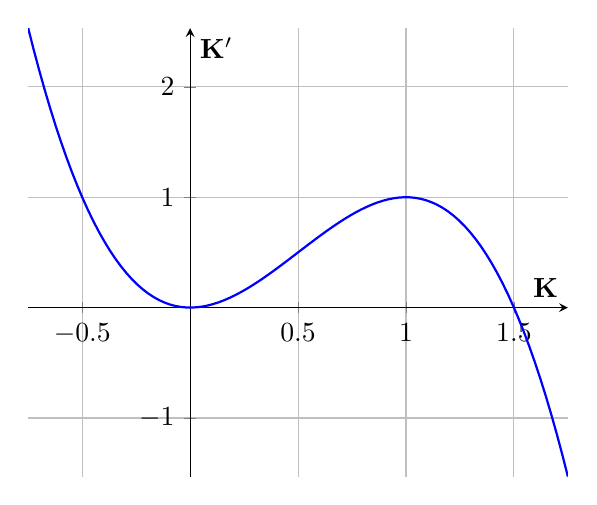
\begin{tikzpicture}
        \begin{axis}[
                axis lines = middle,
                xlabel = {$\vK$},
                ylabel = {$\vK'$},
                domain=-0.75:1.75,
                samples=100,
                grid=both,
            ]
            \addplot[
                color=blue,
                thick
            ]{3*x^2-2*x^3};
        \end{axis}
    \end{tikzpicture}
    \caption{Plot of $\vK' = 3 \vK^2 - 2 \vK^3$ in the case $\vK$ is scalar.}
    \label{fig:plot-g}
\end{figure}

In general, we place no restrictions on the matrix $\vK \in \mathbb{R}^{m \times m}$, hence it might not be diagonalizable directly. It is well known, however, that for every square matrix $\vK$ there exists an invertible matrix $\vP$ such that
\begin{align*}
    \vK = \vP \vJ \vP^{-1}
\end{align*}
where $\vJ \in \mathbb{C}^{m \times m}$ is the Jordan Normal form \cite{jordan-form} of $\vK \in \mathbb{R}^{m \times m}$. From this the dual problem
\begin{align*}
    \vJ = 3 \vJ^2 - 2 \vJ^3
\end{align*}
can be constructed. The block-diagonal structure of $\vJ$ imposes up to four equations per eigenvalue of $\vK$ (see Appendix \ref{app:jordan}):
\begin{align}
    \lambda & = 3\lambda^2 - 2\lambda^3 & \label{eq:cond1}                                   \\
    1       & = 6\lambda - 6\lambda^2   & \text{Only when $d_\lambda\geq2$.}\label{eq:cond2} \\
    0       & = 3 - 6\lambda            & \text{Only when $d_\lambda\geq3$.}\label{eq:cond3} \\
    0       & = 0 - 2                   & \text{Only when $d_\lambda\geq4$.}\label{eq:cond4}
\end{align}
where $d_\lambda$ denote the algebraic multiplicity of eigenvalue $\lambda$ of $\vK$. Clearly, this system of equations is inconsistent when $d_{\lambda} \geq 2$, hence geometric multiplicity of every eigenvalue must also be exactly 1. Together this implies that $\vJ$ is diagonalizable for any fixed point $\vK$. Furthermore, the solutions which satisfy only eq. \ref{eq:cond1} are
\begin{align*}
    \lambda \in \{0, 0.5, 1\}
\end{align*}
hence any fixed point of $\vK = 3 \vK^2 - 2 \vK^3$ must have eigenvalues in this set. Consequently, all idempotent matrices are fixed points, but there exists also non-idempotent fixed points.

Although the initial derivation of $g(\vK) = 3 \vK^2 - 2 \vK^3$ relies on $\vK$ being near-idempotent to the first order, we consider more generally the behaviour of $g$ around the fixed points when applied repeatedly as a recurrence relation. Note first that $h(\lambda) = 3\lambda^2 - 2\lambda^3$ has derivative $h'(\lambda) = 6\lambda - 6\lambda^2$, and so for each fixed point of $g$ we have
\begin{align*}
    h'(0) = 0, \quad h'(0.5) = 1.5, \quad h'(1) = 0.
\end{align*}

Since $|h'(\lambda)| < 1$ for $\lambda \in \{0, 1\}$ these points are attracting whilst $|h'(\lambda)| > 1$ for $\lambda = 0.5$, hence this point is repelling. In other words, if the idempotent corrector $g$ applied as a recurrence relation to $\vM$ converges at some point $\vM'$, then $\vM'$ will be approximately idempotent unless $\vM$ has an eigenvalue of exactly $0.5$.

Furthermore, figure \ref{fig:fractal} shows the result of applying the idempotent corrector recursively 10 times for each point on the complex plane. The attracting regions around $0$ and $1$ are large, hence any matrix that is ``reasonably close'' to idempotent will be projected onto a (within machine precision) idempotent matrix.

\begin{figure*}[!htp]
    \centering
    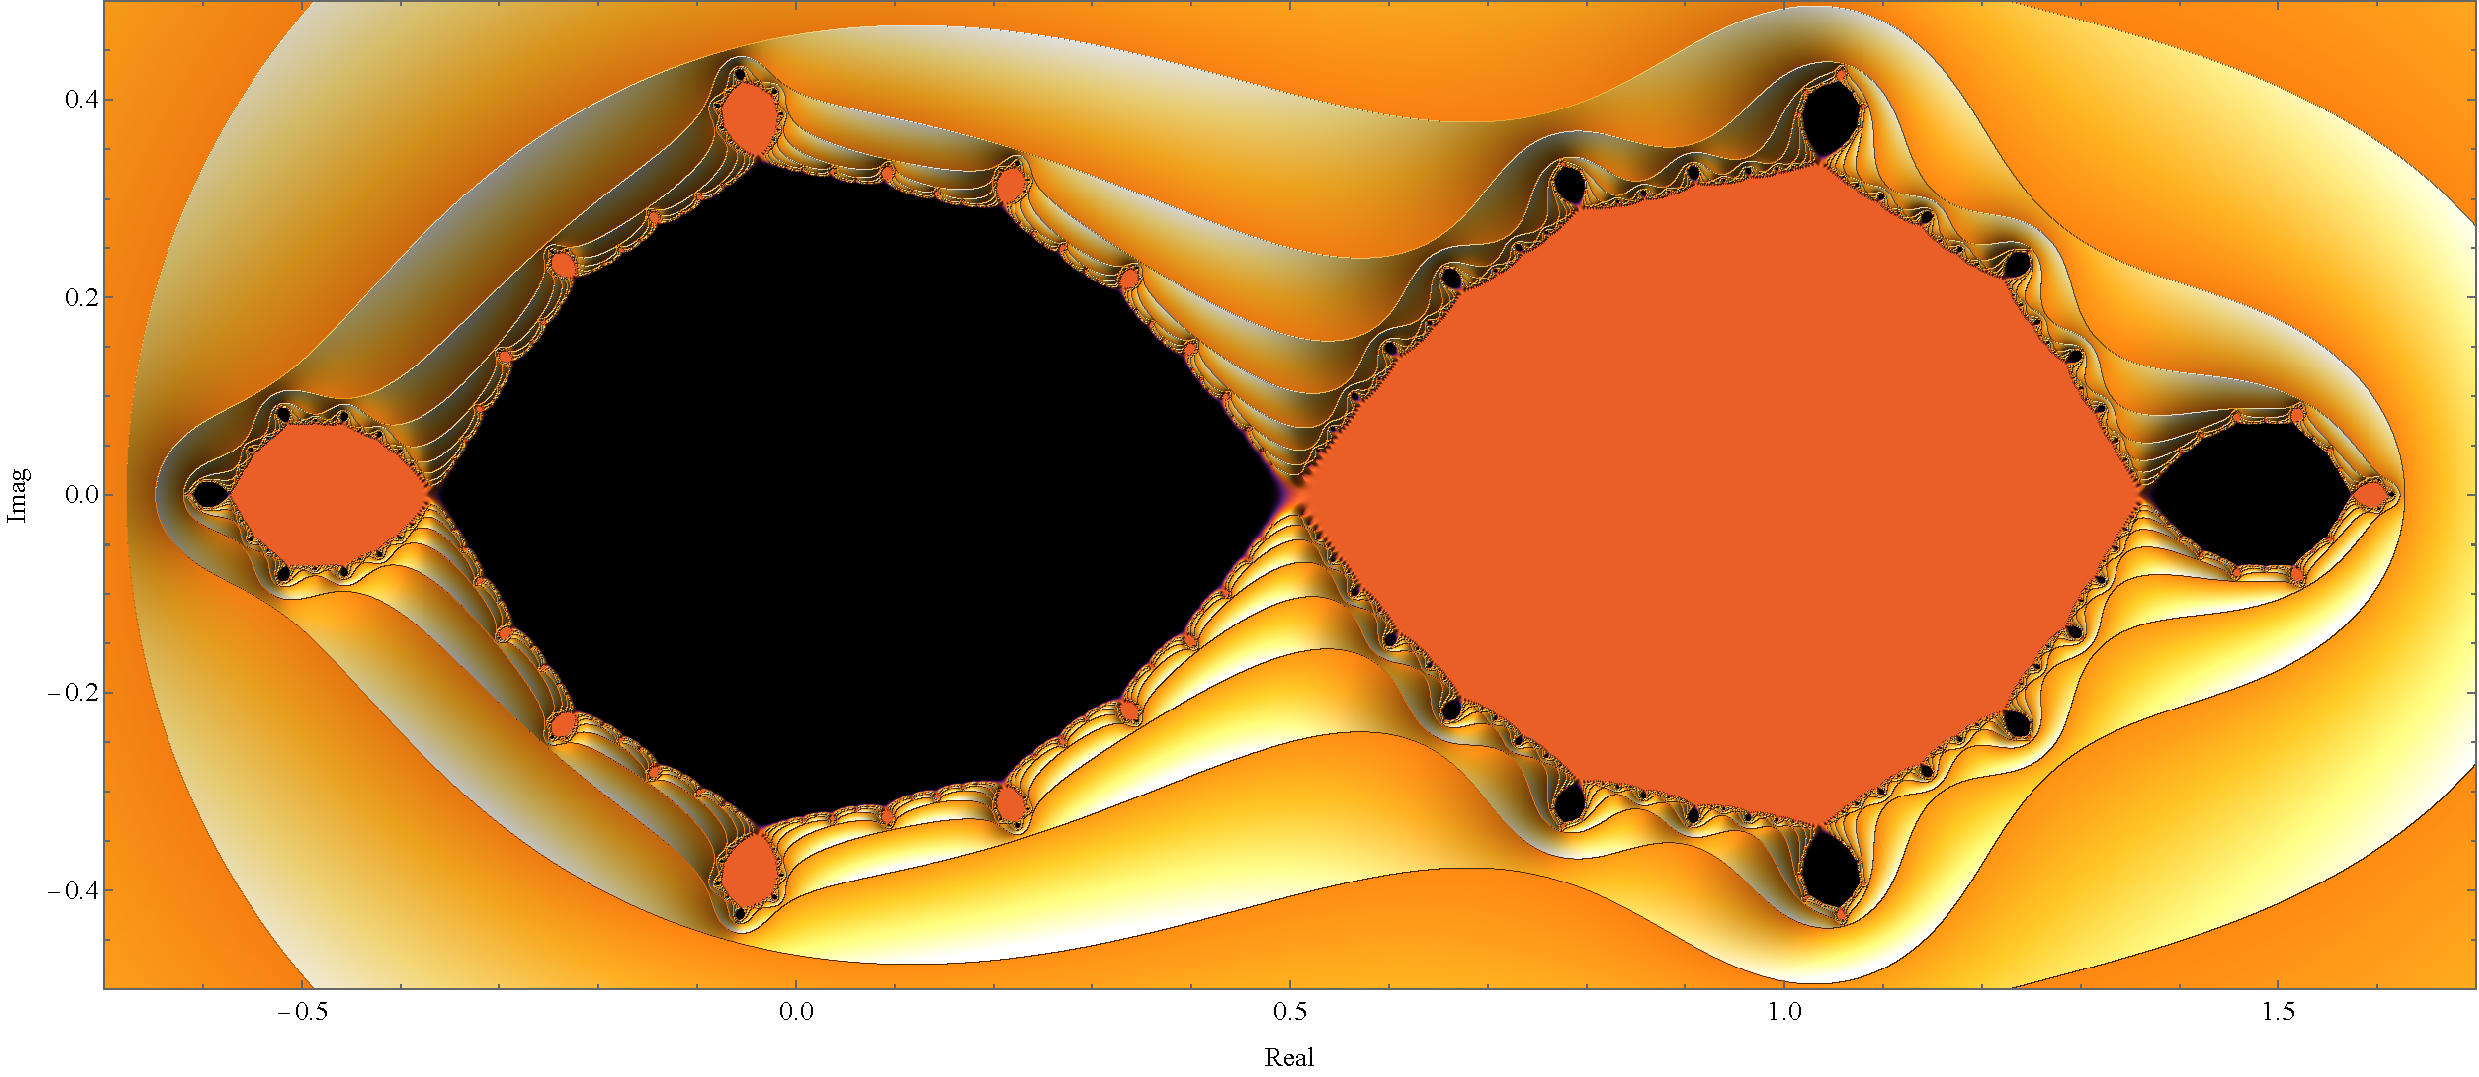
\includegraphics[width=0.99\textwidth]{./resources/fractal.pdf}
    \caption{10-time recursive application of $h(\lambda) = 3\lambda^2 - 2\lambda^3$ for each point on the complex plane. Black areas denote points converging onto $0$, while orange areas denote points converging onto $1$.}
    \label{fig:fractal}
\end{figure*}



% (1 page)
\subsection{Deriving a Training Scheme}
Gradient-based optimization techniques use the gradient of a non-convex loss function as the directional information used to update the hypothesis at each time step. This highlights a core difference between our approach and conventional gradient-based approaches, since the recurrence relation derived above (and shown in figure \ref{fig:plot-g}) exactly describes the ``direction'' to move in to reduce idempotent error. Out method only evaluates $g$ -- finding its derivative is unimportant.

Consider a neural network $f_{\vtheta}: \mathbb{R}^m \to \mathbb{R}^m$ together with its application to input $\vx \in \mathbb{R}^m$, denoted $\vy = f_{\vtheta}(\vx)$. We might then consider the recurrence relation above in the following form:
%
\begin{align*}
    \vy' = 3f_{\vtheta}(\vy) - 2f_{\vtheta}(f_{\vtheta}(\vy))
\end{align*}
%
This describes a desired change in the output of the network which we denote ${\Delta f_{\vtheta}(\vx) = \vy' - \vy}$. In other words, $\Delta f_{\vtheta}(\vx)$ describes the desired change in $\vy$ which moves $\vy$ towards an idempotent projection much in the same way that the quantity $\pd{(-\mathcal{L}(\vy))}{\vy}$ describes the direction which reduces the idempotent loss function $\mathcal{L}(\vy)$ in eq. \ref{eq:idem-loss}. In this work, we therefore define
%
\begin{align}
    \pd{(-\mathcal{L}(\vy))}{\vy} \equiv \Delta f_{\vtheta}(\vx)
    \label{eq:substitution}
\end{align}
%
as an alternative quantity to the traditional, analytical solution to $\pd{(-\mathcal{L}(\vy))}{\vy}$.

To complete the scheme, we consider how a change in the output $\vy$ can be propagated to a change in the parameters $\vtheta$ of $f_{\vtheta}$. This, however, is a straightforward application of the chain rule as it is calculated conventionally in backpropagation.

In practice, the definition \ref{eq:substitution} can be implemented in common machine learning frameworks, such as Jax\footnote{https://github.com/jax-ml/jax} and PyTorch\footnote{https://pytorch.org} as a user-defined automatic differentiation rule (see Appendix \ref{app:autodiff-rule}).

\begin{figure}[h]
    \centering
    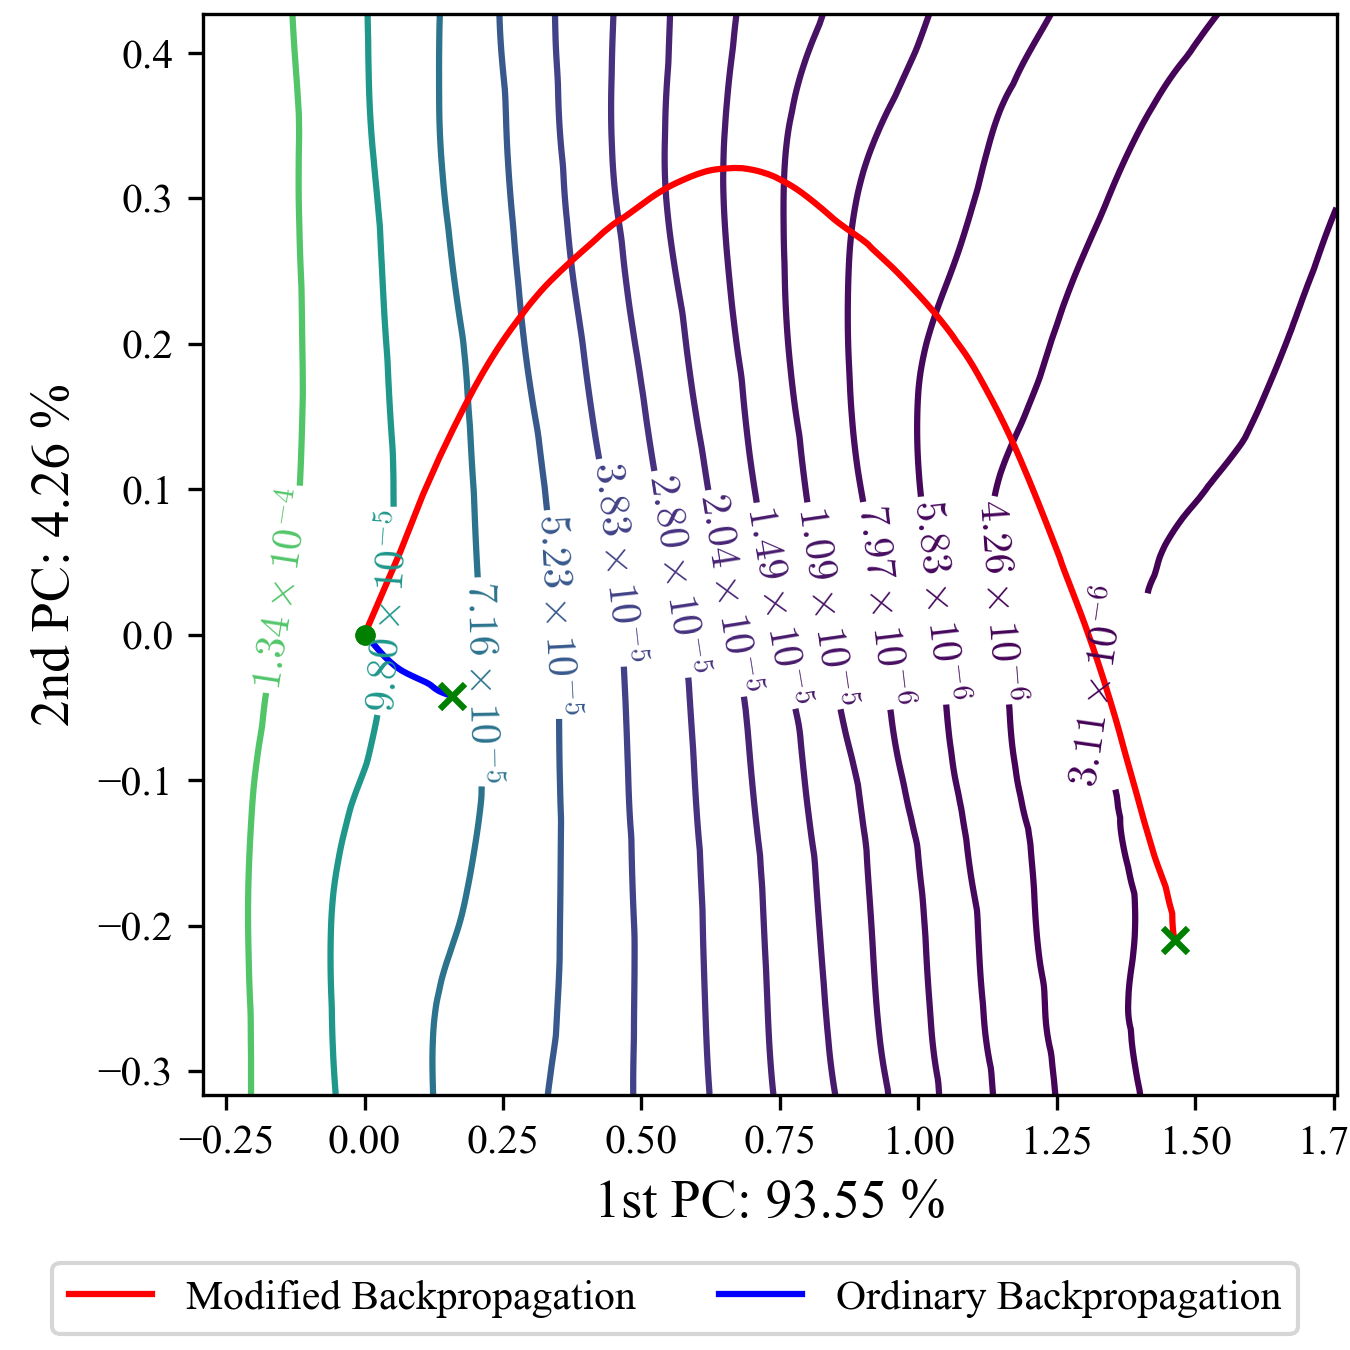
\includegraphics[width=0.95\columnwidth]{./resources/pca_b2.png}
    \label{fig:pca-b2}
    \caption{PCA analysis and projected optimizer trajectories for network B2.}
\end{figure}

\begin{figure}[h]
    \centering
    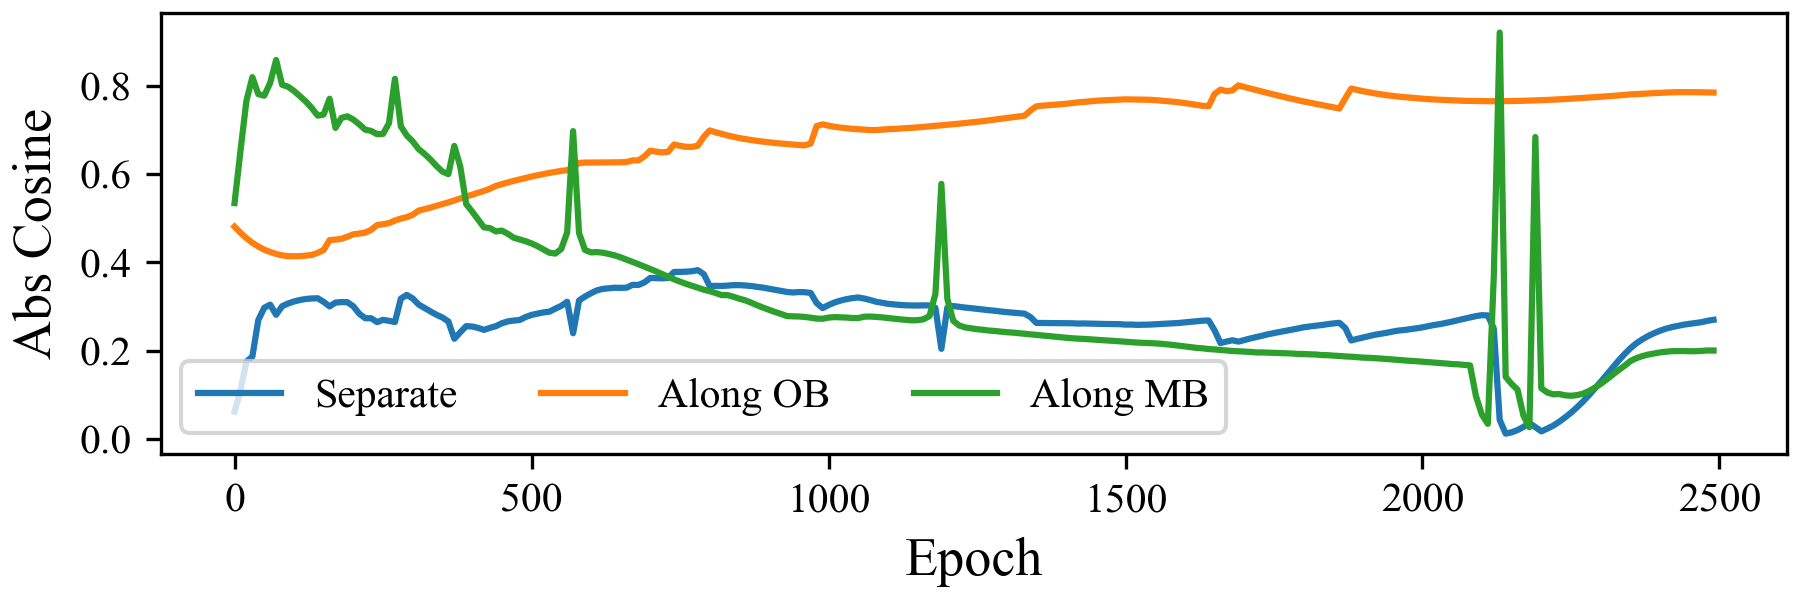
\includegraphics[width=0.95\columnwidth]{./resources/cos.png}
    \label{fig:cos-b2}
    \caption{Cosine similarity of gradients over time of a representative training run with model B2.}
\end{figure}

\begin{figure}[h]
    \centering
    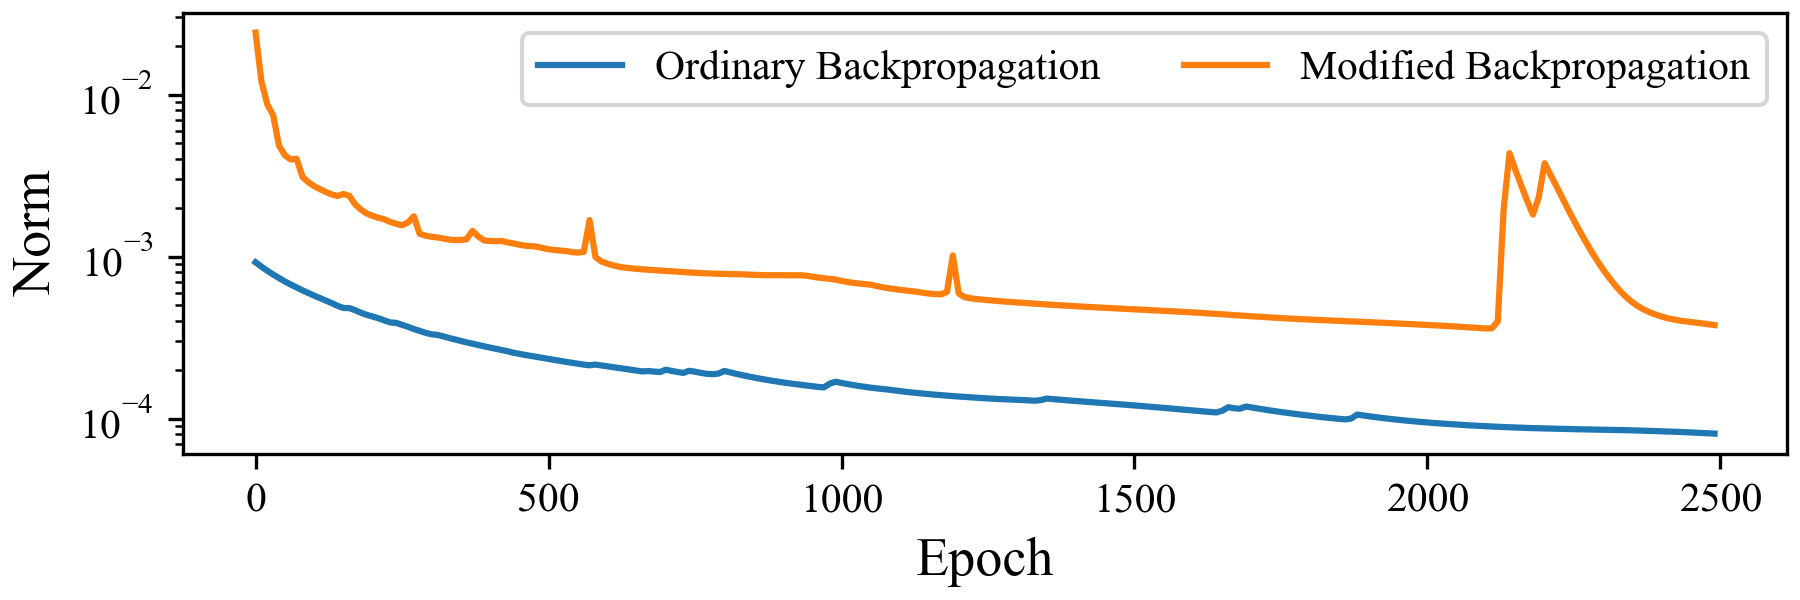
\includegraphics[width=0.95\columnwidth]{./resources/norm.png}
    \label{fig:norm-b2}
    \caption{Norm of gradients over time of a representative training run with model B2.}
\end{figure}

% (3 pages)
\section{Experimental Results}
\label{sec:experiment}
%\textit{On experimental networks we give line graphs comparing absolute error at varying learning rates. We also give line graphs for LRs over many epochs. Takeaway message is that for deeper/wider networks we outperform ordinary autodiff by a lot.}
% Outline differences in training scheme.
% Error across LR for B3&B4
% Error across Runs for B3&B4
% (PCA analysis graphs)
To evaluate the training scheme suggested in section \ref{sec:method} we compare relative performance between the two methods: ``Ordinary Backpropagation'' with the quantity $\pd{(-\mathcal{L}(\vy))}{\vy}$ resolved at runtime by automatic differentiation, and ``Modified Backpropagation'' with the modified backpropagation rule for $\pd{(-\mathcal{L}(\vy))}{\vy}$. To demonstrate the flexibility of the approach, we report results for four diverse MLP-style networks, as described in table \ref{tab:networks}.

\begin{table}[htbp]
    \begin{center}
        \begin{tabular}{|c|p{0.18\textwidth}|c|}
            \hline
            \textbf{Identifier} & \textbf{Architecture}                                                                                                    & \textbf{No. Parameters} \\
            \hline
            \hline
            B1                  & Linear(5,5)                                                                                                              & $30$                    \\
            \hline
            B2                  & Linear(128, 256) \newline Linear(256, 256) \newline Linear(256, 256) \newline Linear(256, 256) \newline Linear(256, 128) & $263\,296$              \\
            \hline
            B3                  & Linear(4096, 1024) \newline Linear(1024, 4096)                                                                           & $8\,393\,728$           \\
            \hline
            B4                  & Linear(784, 1024) \newline Linear(1024, 2048) \newline Linear(2048, 784)                                                 & $4\,509\,456$           \\
            \hline
        \end{tabular}
        \vspace{5pt}
        \caption{Four neural networks for testing. Each ``Linear($n$, $m$)'' block is parameterized by its input dimension $n$ and its output dimension $m$, corresponding to the underlying $\vW \in \mathbb{R}^{n \times m}$ weight matrix. Every block has an associated bias vector and LeakyReLU($0.2$) activation function. B1 represents a trivial network, B2 represents a relatively deep network, B3 represents a relatively wide network, and B4 represents a practically useful network.}
        \label{tab:networks}
    \end{center}
\end{table}

The dataset used for training in this section is drawn from a normal distribution with mean $0$ and standard deviation $1$. To prevent concerns about overfitting, the distribution is sampled i.i.d. at each epoch during training. Furthermore, a batch size of $1000$ is used, although comparable results have been found using batch sizes between $32$ and $10\,000$.

Runs which result in null matrices are filtered out (so are identities).

Can we put more results for all networks for tanh and sigmoid in an appendix?

\begin{figure*}[htbp]
    \centering
    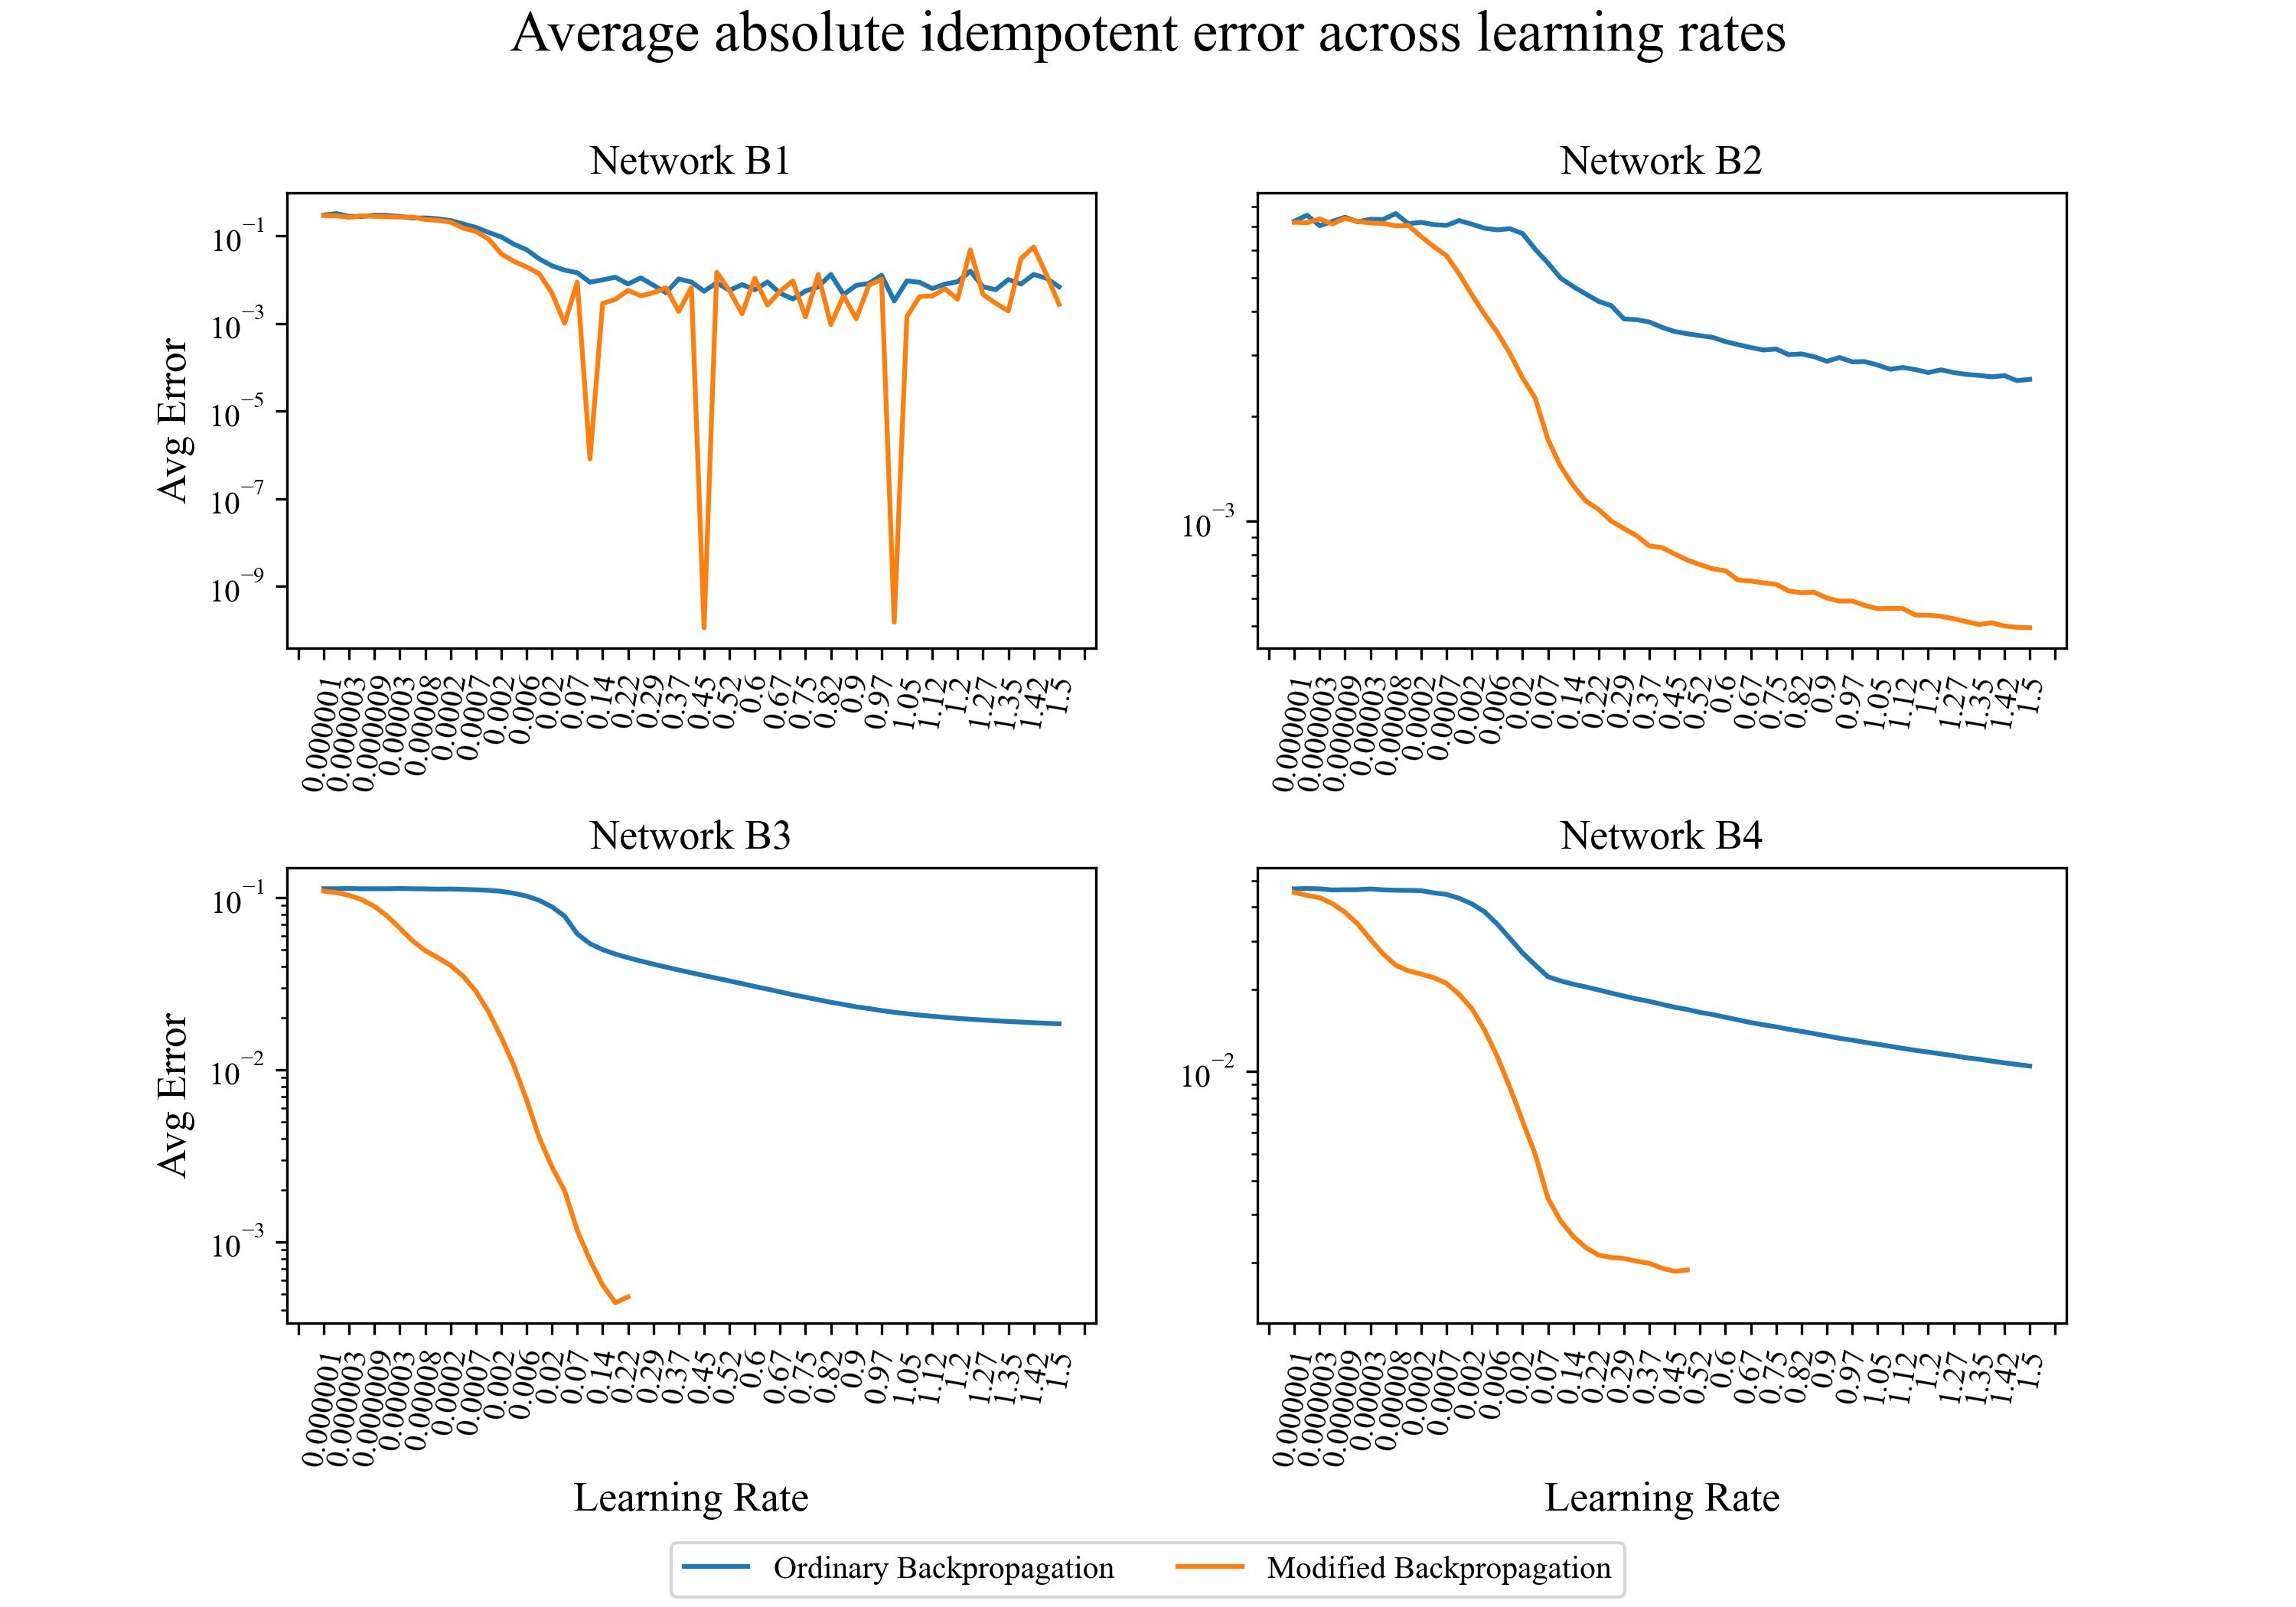
\includegraphics[width=\textwidth]{./resources/abs_err_b1234.png}
    \label{fig:avg-abs-err}
    \caption{Average of 10 runs of each algorithm for a variety of learning rates. Networks are randomly initialized and trained for $2\,500$ epochs. Runs which did not return a solution with lower idempotent error than the initial value are discarded, and the average is over remaining runs. For networks B3 and B4, learning rates $>0.22$ and $>0.52$ respectively had no runs with improvement in error. For ``Modified Backpropagation'' on B1, some runs resulted in approximately $\bm{0}$ which, due to floating-point imprecision, results in the error spikes.}
\end{figure*}

\begin{figure*}[htbp]
    \centering
    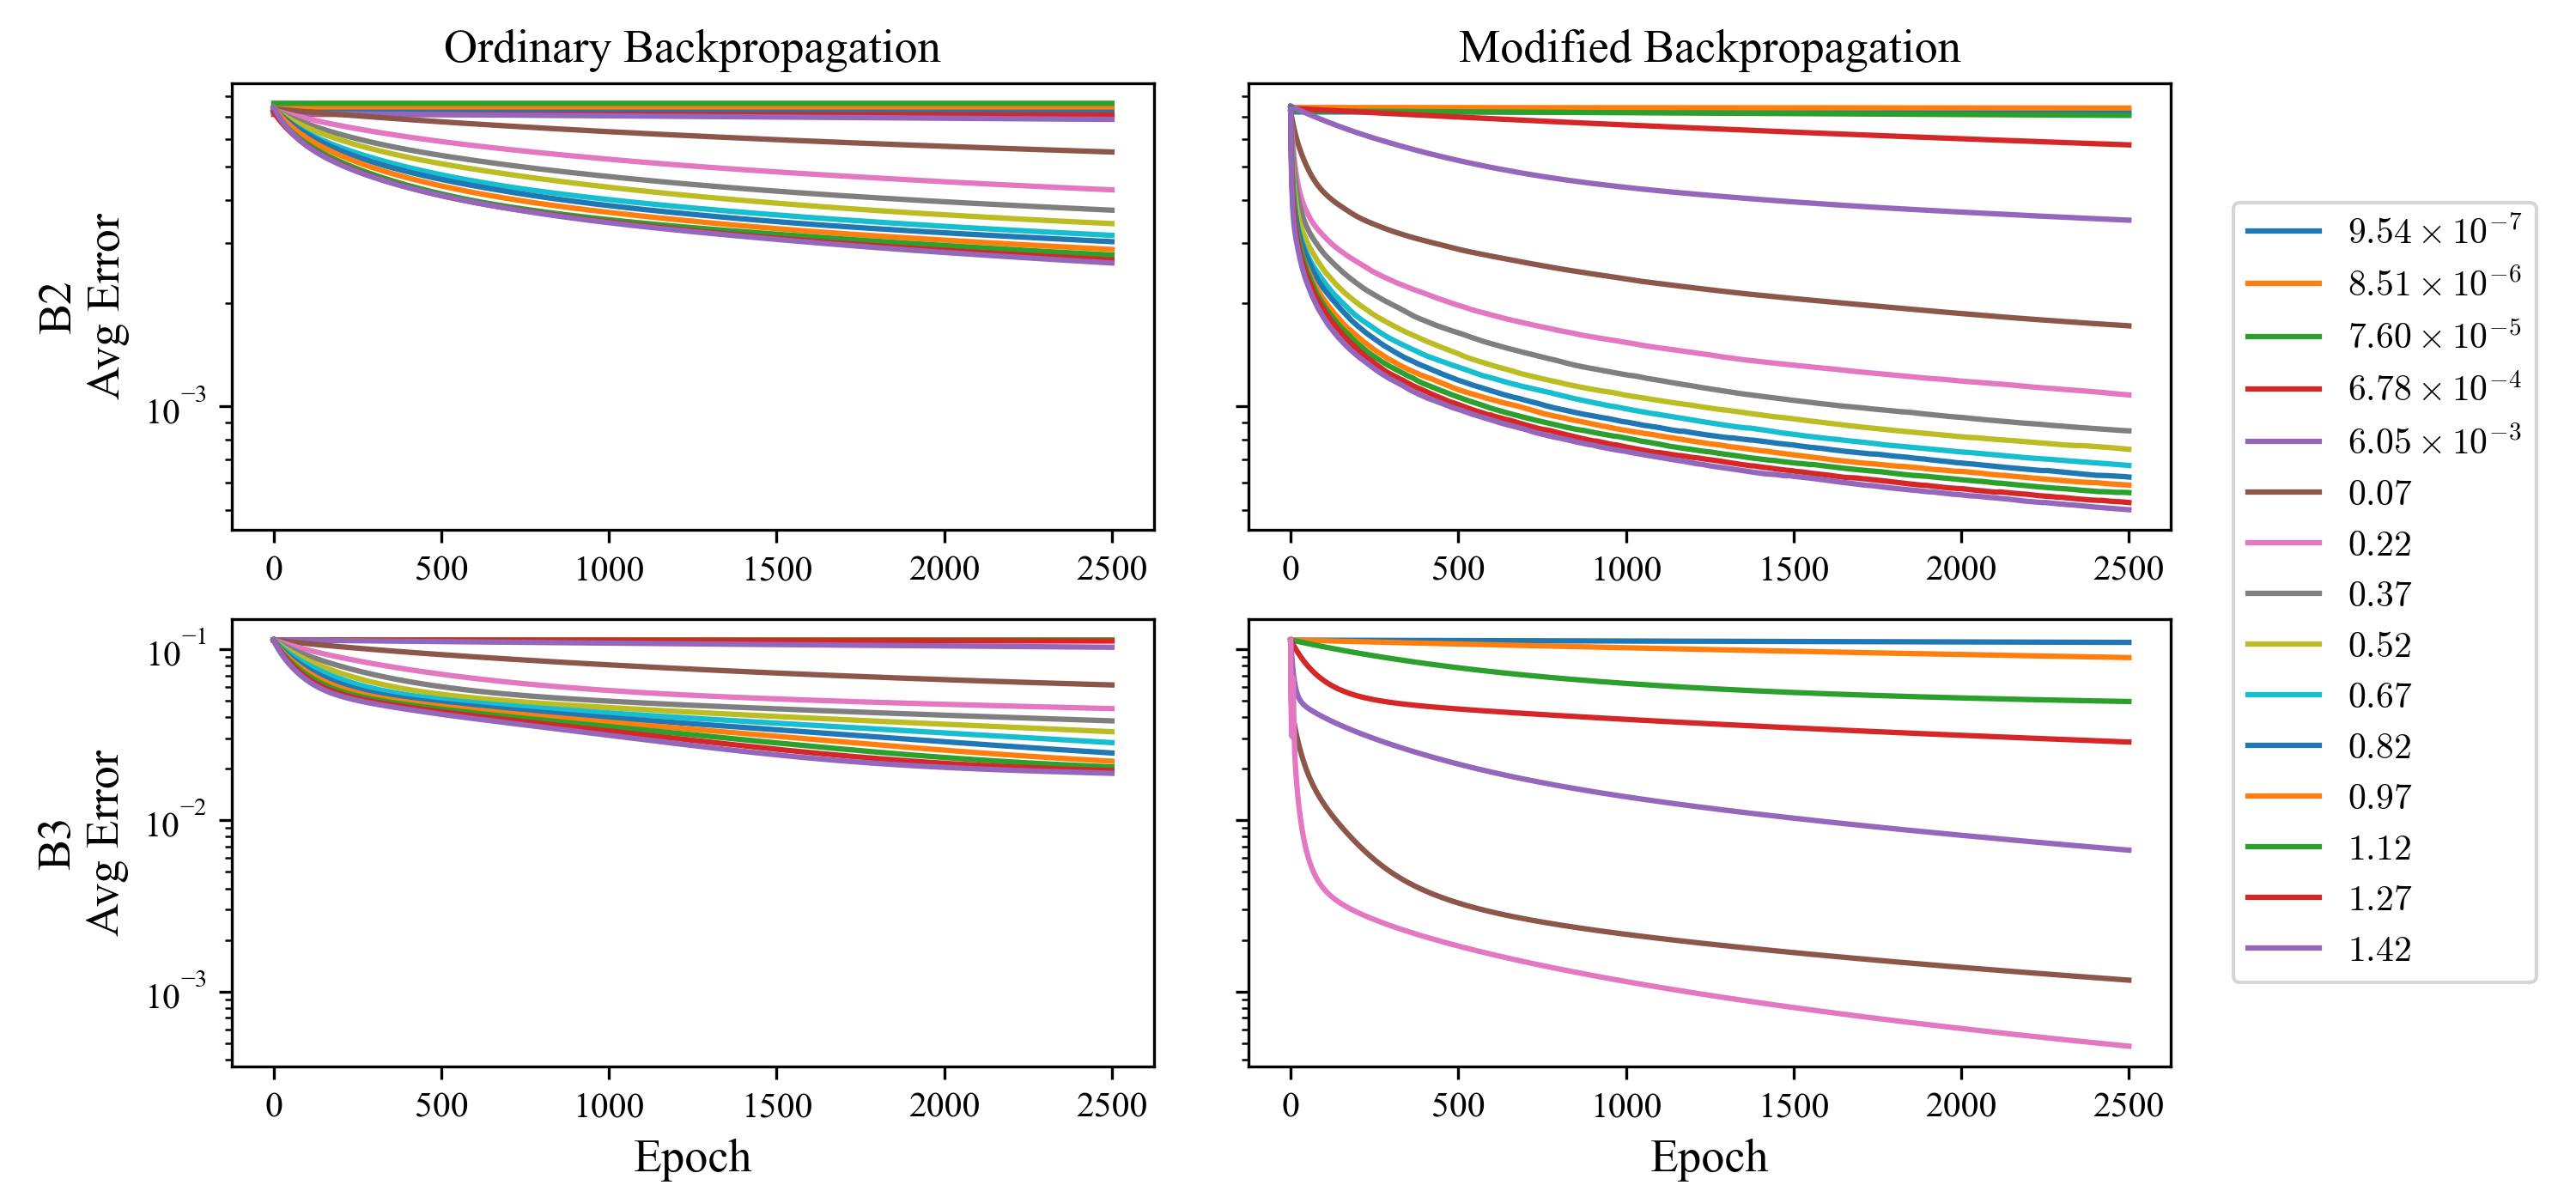
\includegraphics[width=\textwidth]{./resources/runs_err_b23.png}
    \label{fig:avg-epoch-err}
    \caption{On networks B2 and B3, the average idempotent error across 10 runs for each learning rate is reported for each algorithm. Each column of graphs represents one algorithm. ``Modified Backpropagation'' achieves lower idempotent error at lower learning rates than ``Ordinary Backpropagation''.}
\end{figure*}

\textit{TODO: Include a section on qualitative differences in behaviour of modified and ordinary backpropagation. Does one method travel a different route in the loss landscape? This small section is to be suggestive of distinguishing features of the new method.}

\subsection{Application to Generative Networks}
%\textit{We replicate the results of IGN on MNIST and CelebA. Latent space analysis. Takeaway is that we show application to a U-net GAN architecture based on Conv layers.}

\begin{figure*}[htbp]
    \centering
    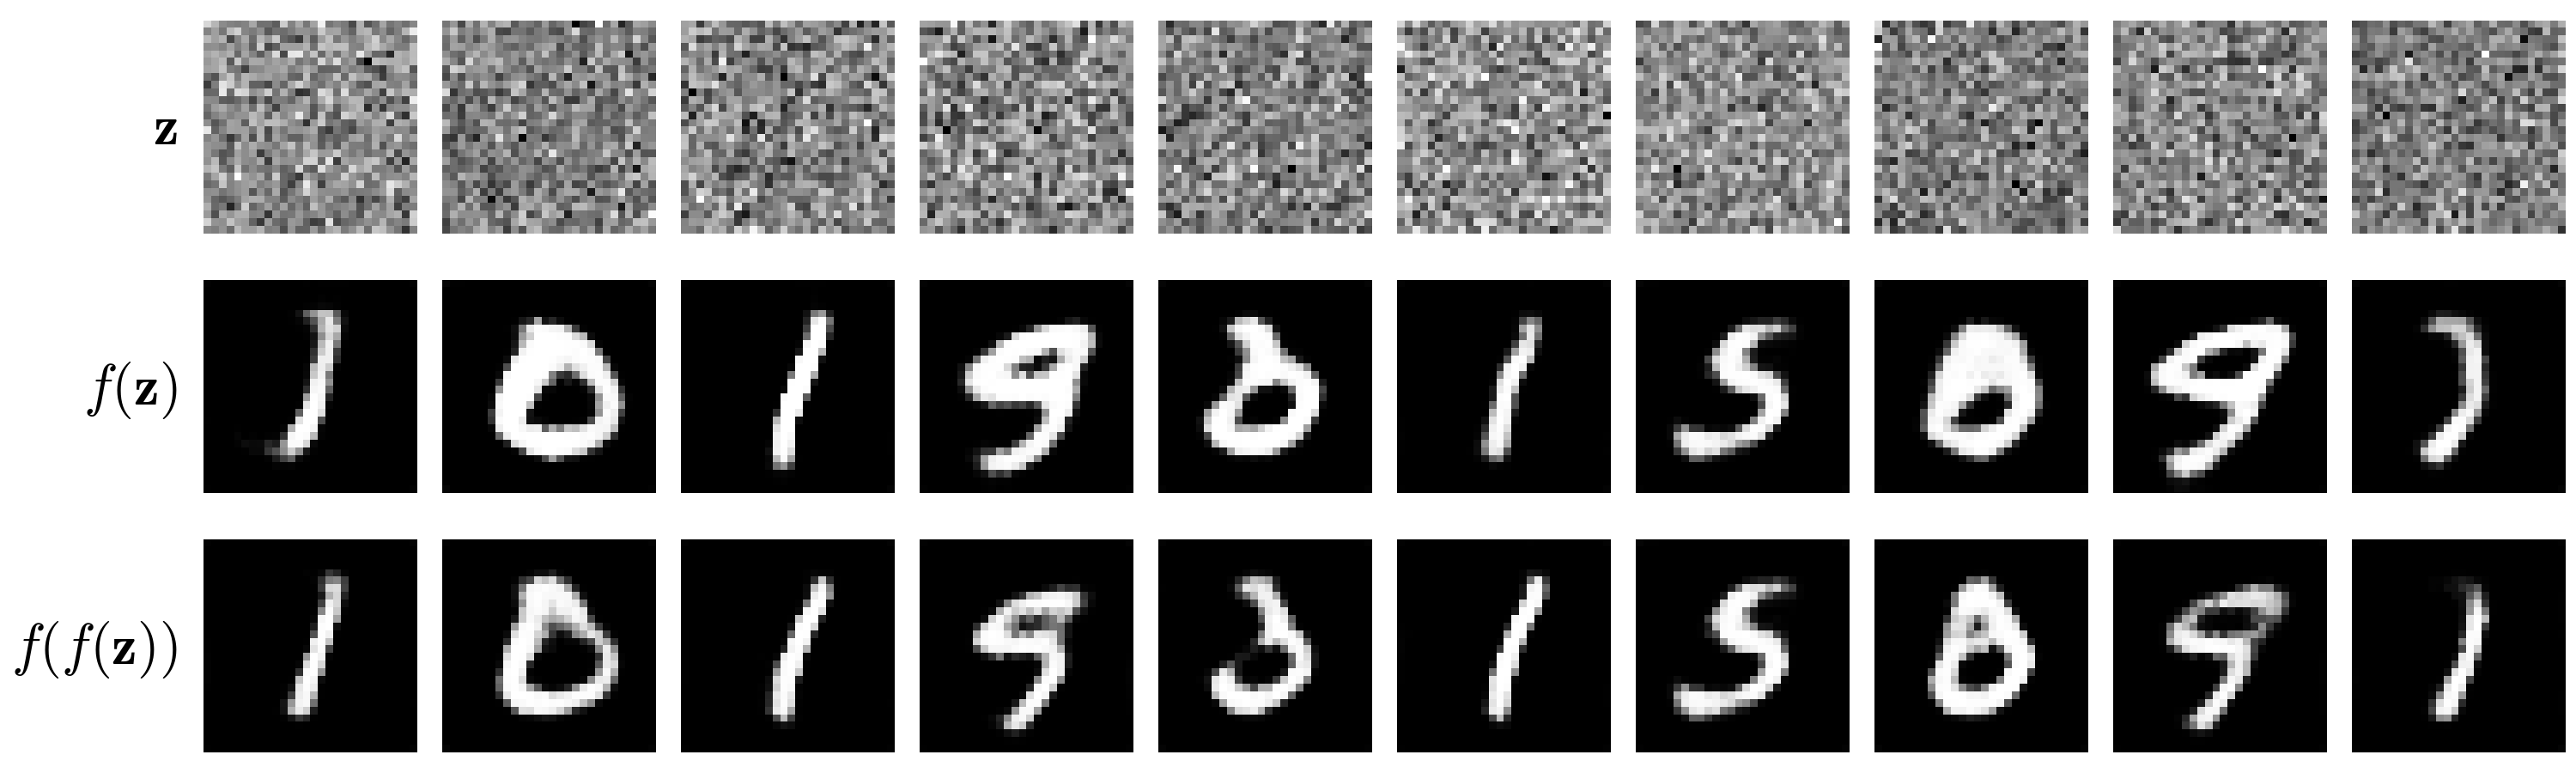
\includegraphics[width=\textwidth]{./resources/modified_0-1_0-1_rand_noise_mapping.png}
    \label{fig:gen-mnist}
    \caption{U-DCGAN architecture trained on MNIST. Random noise mappings.}
\end{figure*}


\begin{figure*}[htbp]
    \centering
    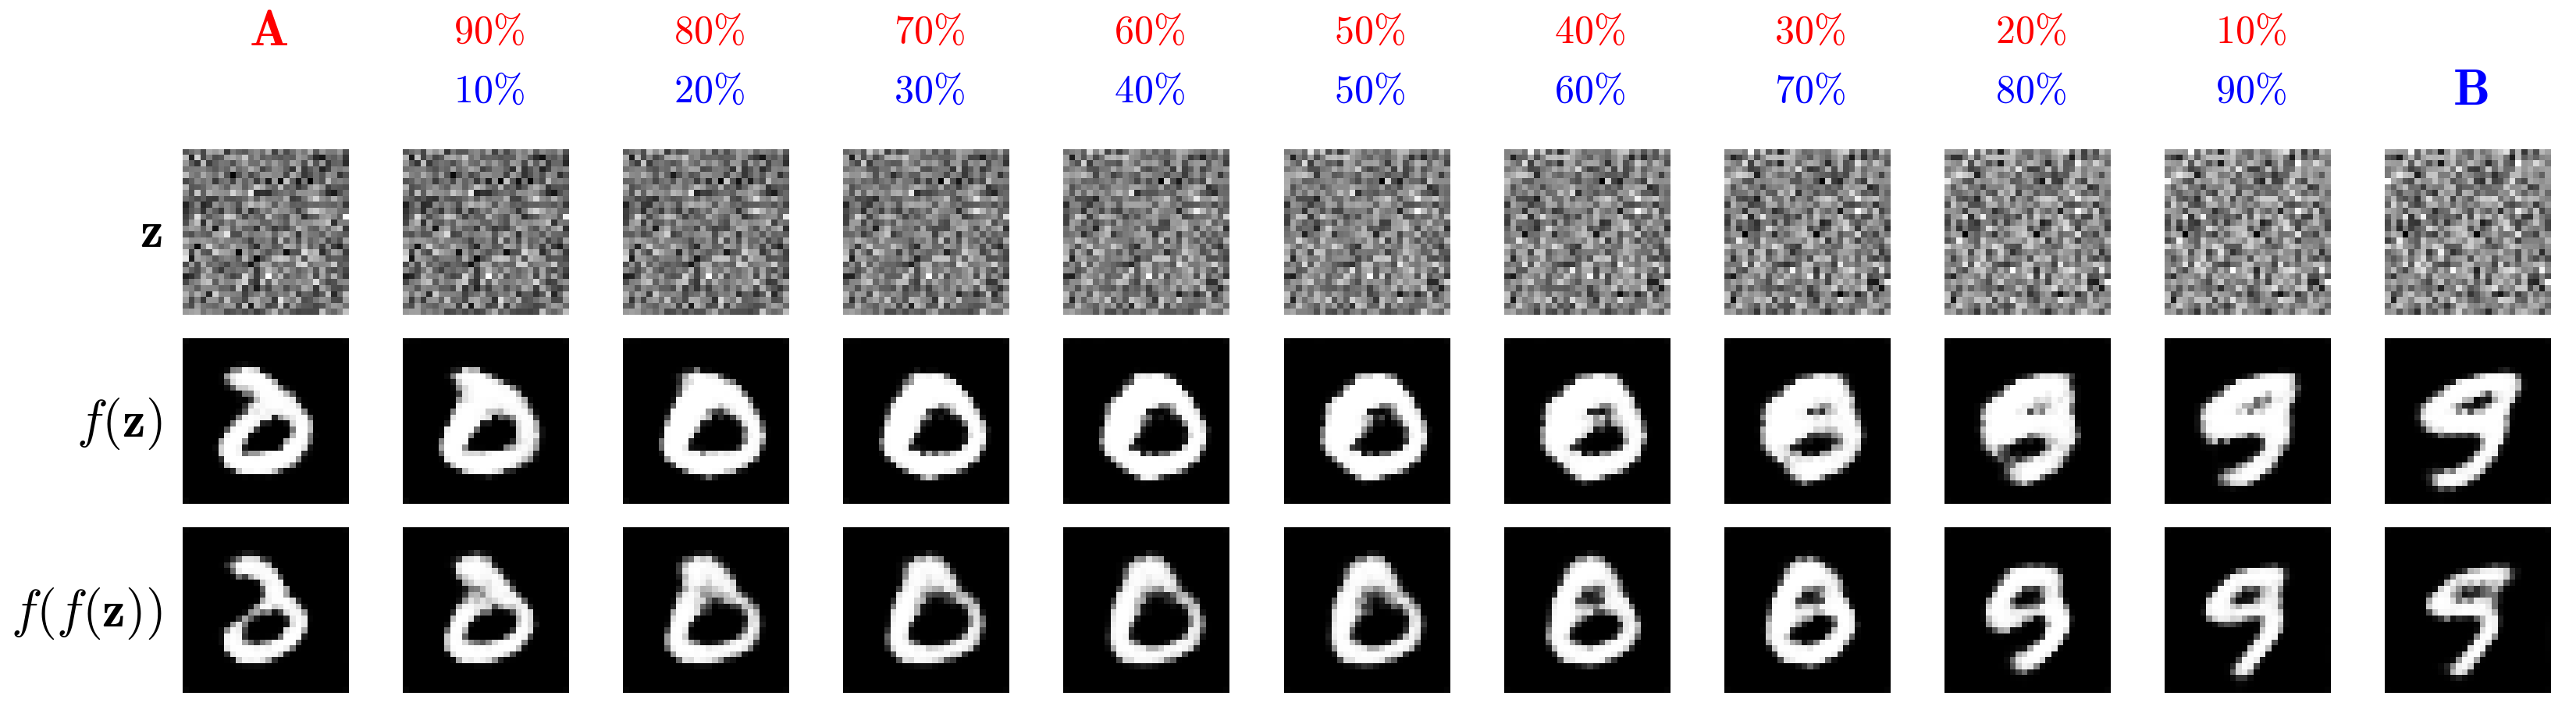
\includegraphics[width=\textwidth]{./resources/modified_0-1_0-1_rand_latent_space.png}
    \label{fig:latent-mnist}
    \caption{U-DCGAN architecture trained on MNIST. Latent space linear interpolation.}
\end{figure*}

%\begin{figure}
%    \centering     %%% not \center
%    \subfigure[Modified Backpropagation]{
%        \label{fig:gen-mnist-a}
%        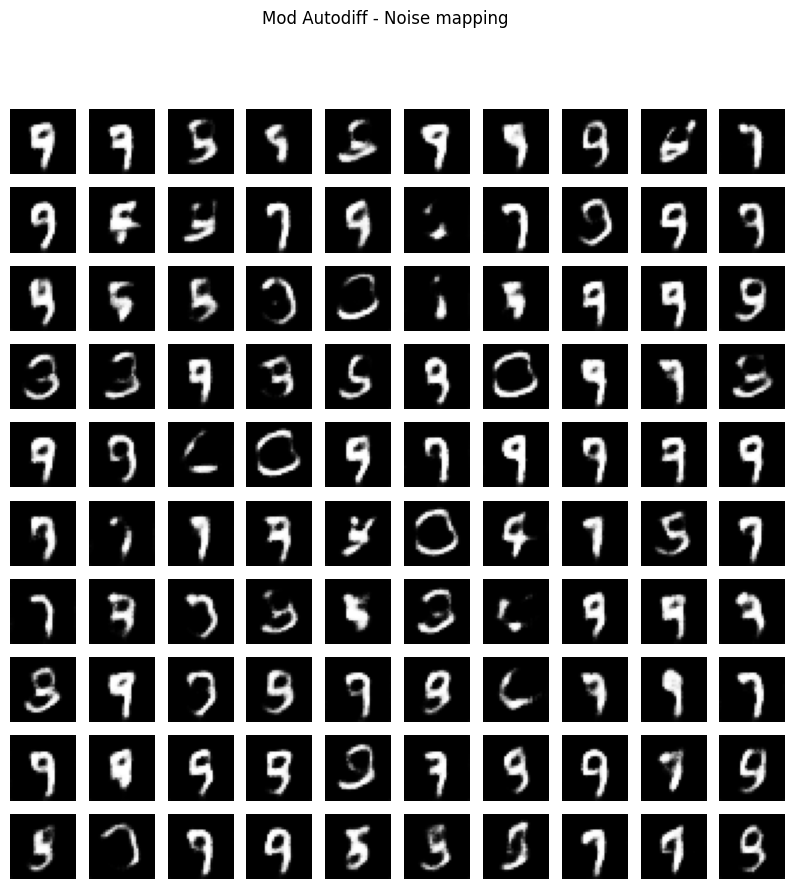
\includegraphics[width=0.9\columnwidth]{./resources/mnist-mod-autodiff-generative.png}
%    }
%    \subfigure[Ordinary Backpropagation]{
%        \label{fig:gen-mnist-b}
%        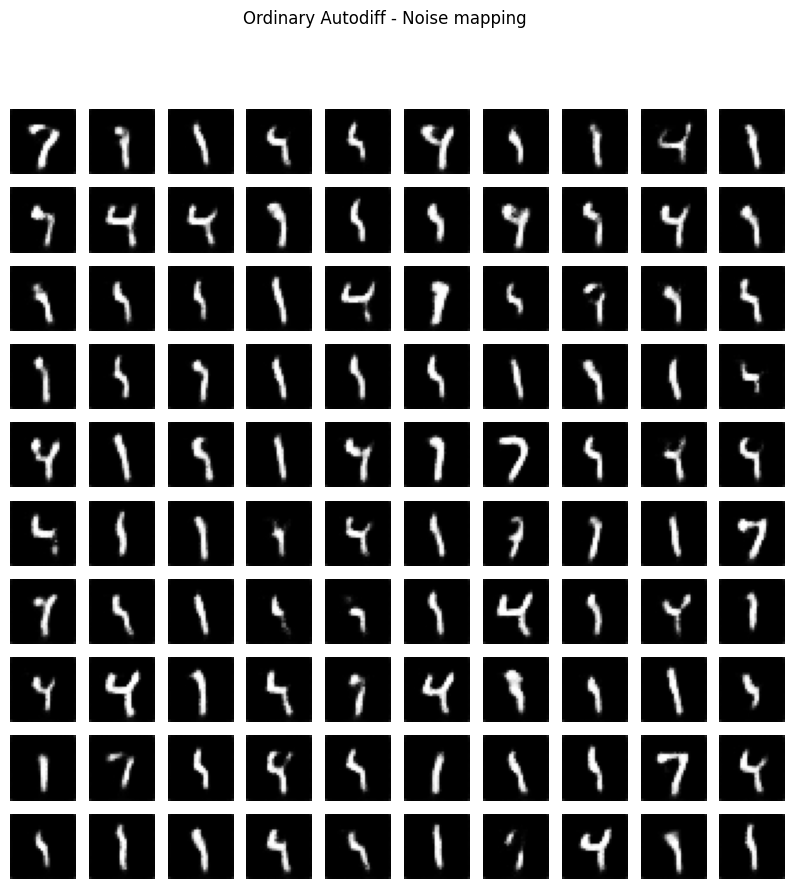
\includegraphics[width=0.9\columnwidth]{./resources/mnist-ord-autodiff-generative.png}
%    }
%    \caption{U-DCGAN architecture trained on MNIST.}
%    \label{fig:gen-mnist}
%\end{figure}

\textit{TODO: Trim the above graph, no need to show 100 samples for each model.}

\textit{TODO: Include a similar graph as the above for CelebA dataset.}

\textit{TODO: Produce graph for latent-space analysis and write comments.}


% (0.5 pages)
\section{Related Work}
\label{sec:related}
\textit{Review Idempotent Generative Networks, contrasting our work on a gradient-free approach. Have others applied perturbation theory to ML? We suffer same problems as GANs: mode collapse.}

% (0.5 pages)
\section{Conclusion}
\label{sec:conclusion}
\textit{Give a conclusion of central idea: the use of perturbation analysis to find an iterator which we have successfully applied to a range of toy examples and GAN scenarios.}

% Acknowledgements should only appear in the accepted version.
\section*{Acknowledgements}

\textbf{Do not} include acknowledgements in the initial version of
the paper submitted for blind review.

If a paper is accepted, the final camera-ready version can (and
usually should) include acknowledgements.  Such acknowledgements
should be placed at the end of the section, in an unnumbered section
that does not count towards the paper page limit. Typically, this will
include thanks to reviewers who gave useful comments, to colleagues
who contributed to the ideas, and to funding agencies and corporate
sponsors that provided financial support.

\section*{Impact Statement}

Authors are \textbf{required} to include a statement of the potential
broader impact of their work, including its ethical aspects and future
societal consequences. This statement should be in an unnumbered
section at the end of the paper (co-located with Acknowledgements --
the two may appear in either order, but both must be before References),
and does not count toward the paper page limit. In many cases, where
the ethical impacts and expected societal implications are those that
are well established when advancing the field of Machine Learning,
substantial discussion is not required, and a simple statement such
as the following will suffice:

``This paper presents work whose goal is to advance the field of
Machine Learning. There are many potential societal consequences
of our work, none which we feel must be specifically highlighted here.''

The above statement can be used verbatim in such cases, but we
encourage authors to think about whether there is content which does
warrant further discussion, as this statement will be apparent if the
paper is later flagged for ethics review.


% In the unusual situation where you want a paper to appear in the
% references without citing it in the main text, use \nocite
%\nocite{langley00}

\bibliography{bibliography}
\bibliographystyle{icml2025}


%%%%%%%%%%%%%%%%%%%%%%%%%%%%%%%%%%%%%%%%%%%%%%%%%%%%%%%%%%%%%%%%%%%%%%%%%%%%%%%
%%%%%%%%%%%%%%%%%%%%%%%%%%%%%%%%%%%%%%%%%%%%%%%%%%%%%%%%%%%%%%%%%%%%%%%%%%%%%%%
% APPENDIX
%%%%%%%%%%%%%%%%%%%%%%%%%%%%%%%%%%%%%%%%%%%%%%%%%%%%%%%%%%%%%%%%%%%%%%%%%%%%%%%
%%%%%%%%%%%%%%%%%%%%%%%%%%%%%%%%%%%%%%%%%%%%%%%%%%%%%%%%%%%%%%%%%%%%%%%%%%%%%%%
\newpage
\appendix
\onecolumn

\section{Solutions to the ansatz}
\label{app:solutions}
\textit{Show up to some order (approx 10?) the families of solutions to the ansatz when $\vK$ is near-idempotent to the first order. Also give a concrete example (like in your slides) for how we actually compute the corrector.}

\section{Jordan normal form analysis}
\label{app:jordan}
\textit{Give the full Jordan Normal Form analysis.}

\section{Automatic differentiation rule}
\label{app:autodiff-rule}
\textit{Describe the implementation of the autodiff rule in PyTorch. Show the code and the computational graph highlighting the differences between ordinary and modified backpropagation.}

\section{Generative samples}
\label{app:gen-samples}
\begin{figure}[htbp]
    \centering
    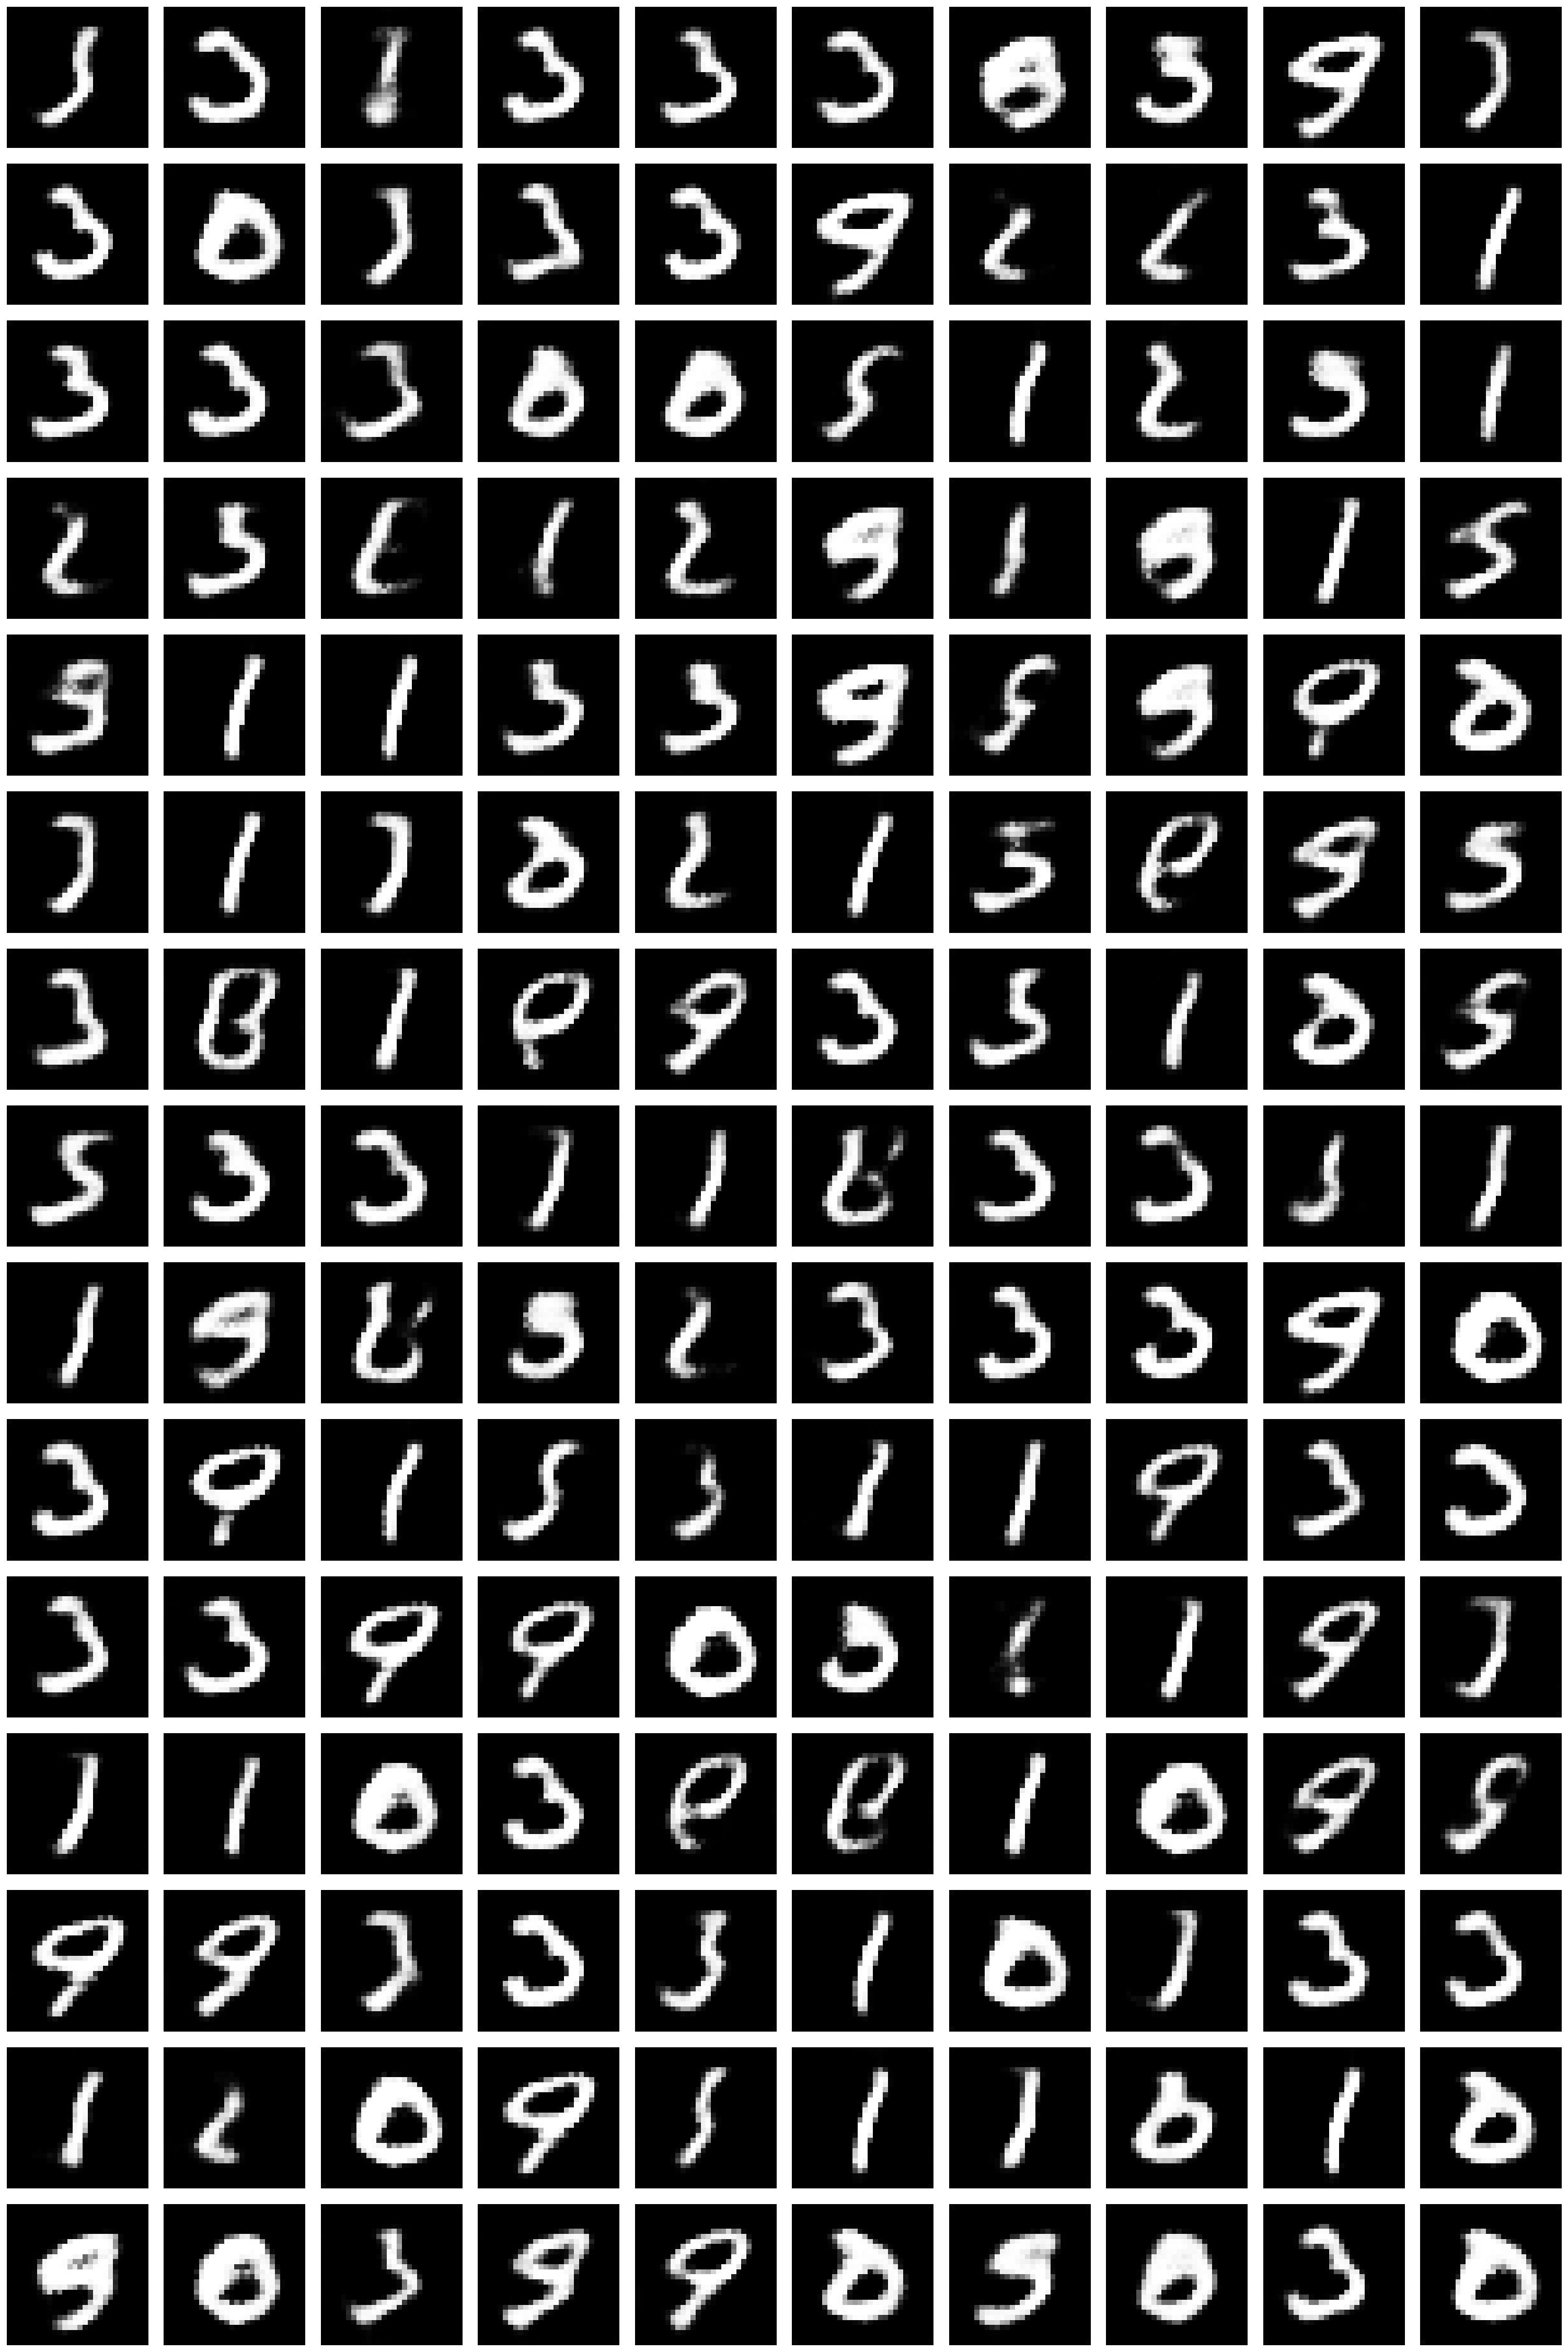
\includegraphics[width=0.8\textwidth]{./resources/modified_0-1_0-1_rand_samples.png}
    \label{fig:big-gen-mnist}
    \caption{U-DCGAN architecture trained on MNIST. 150 random samples.}
\end{figure}

\section{PCA analysis plots}
\label{app:pca}
\begin{figure}[htbp]
    \centering
    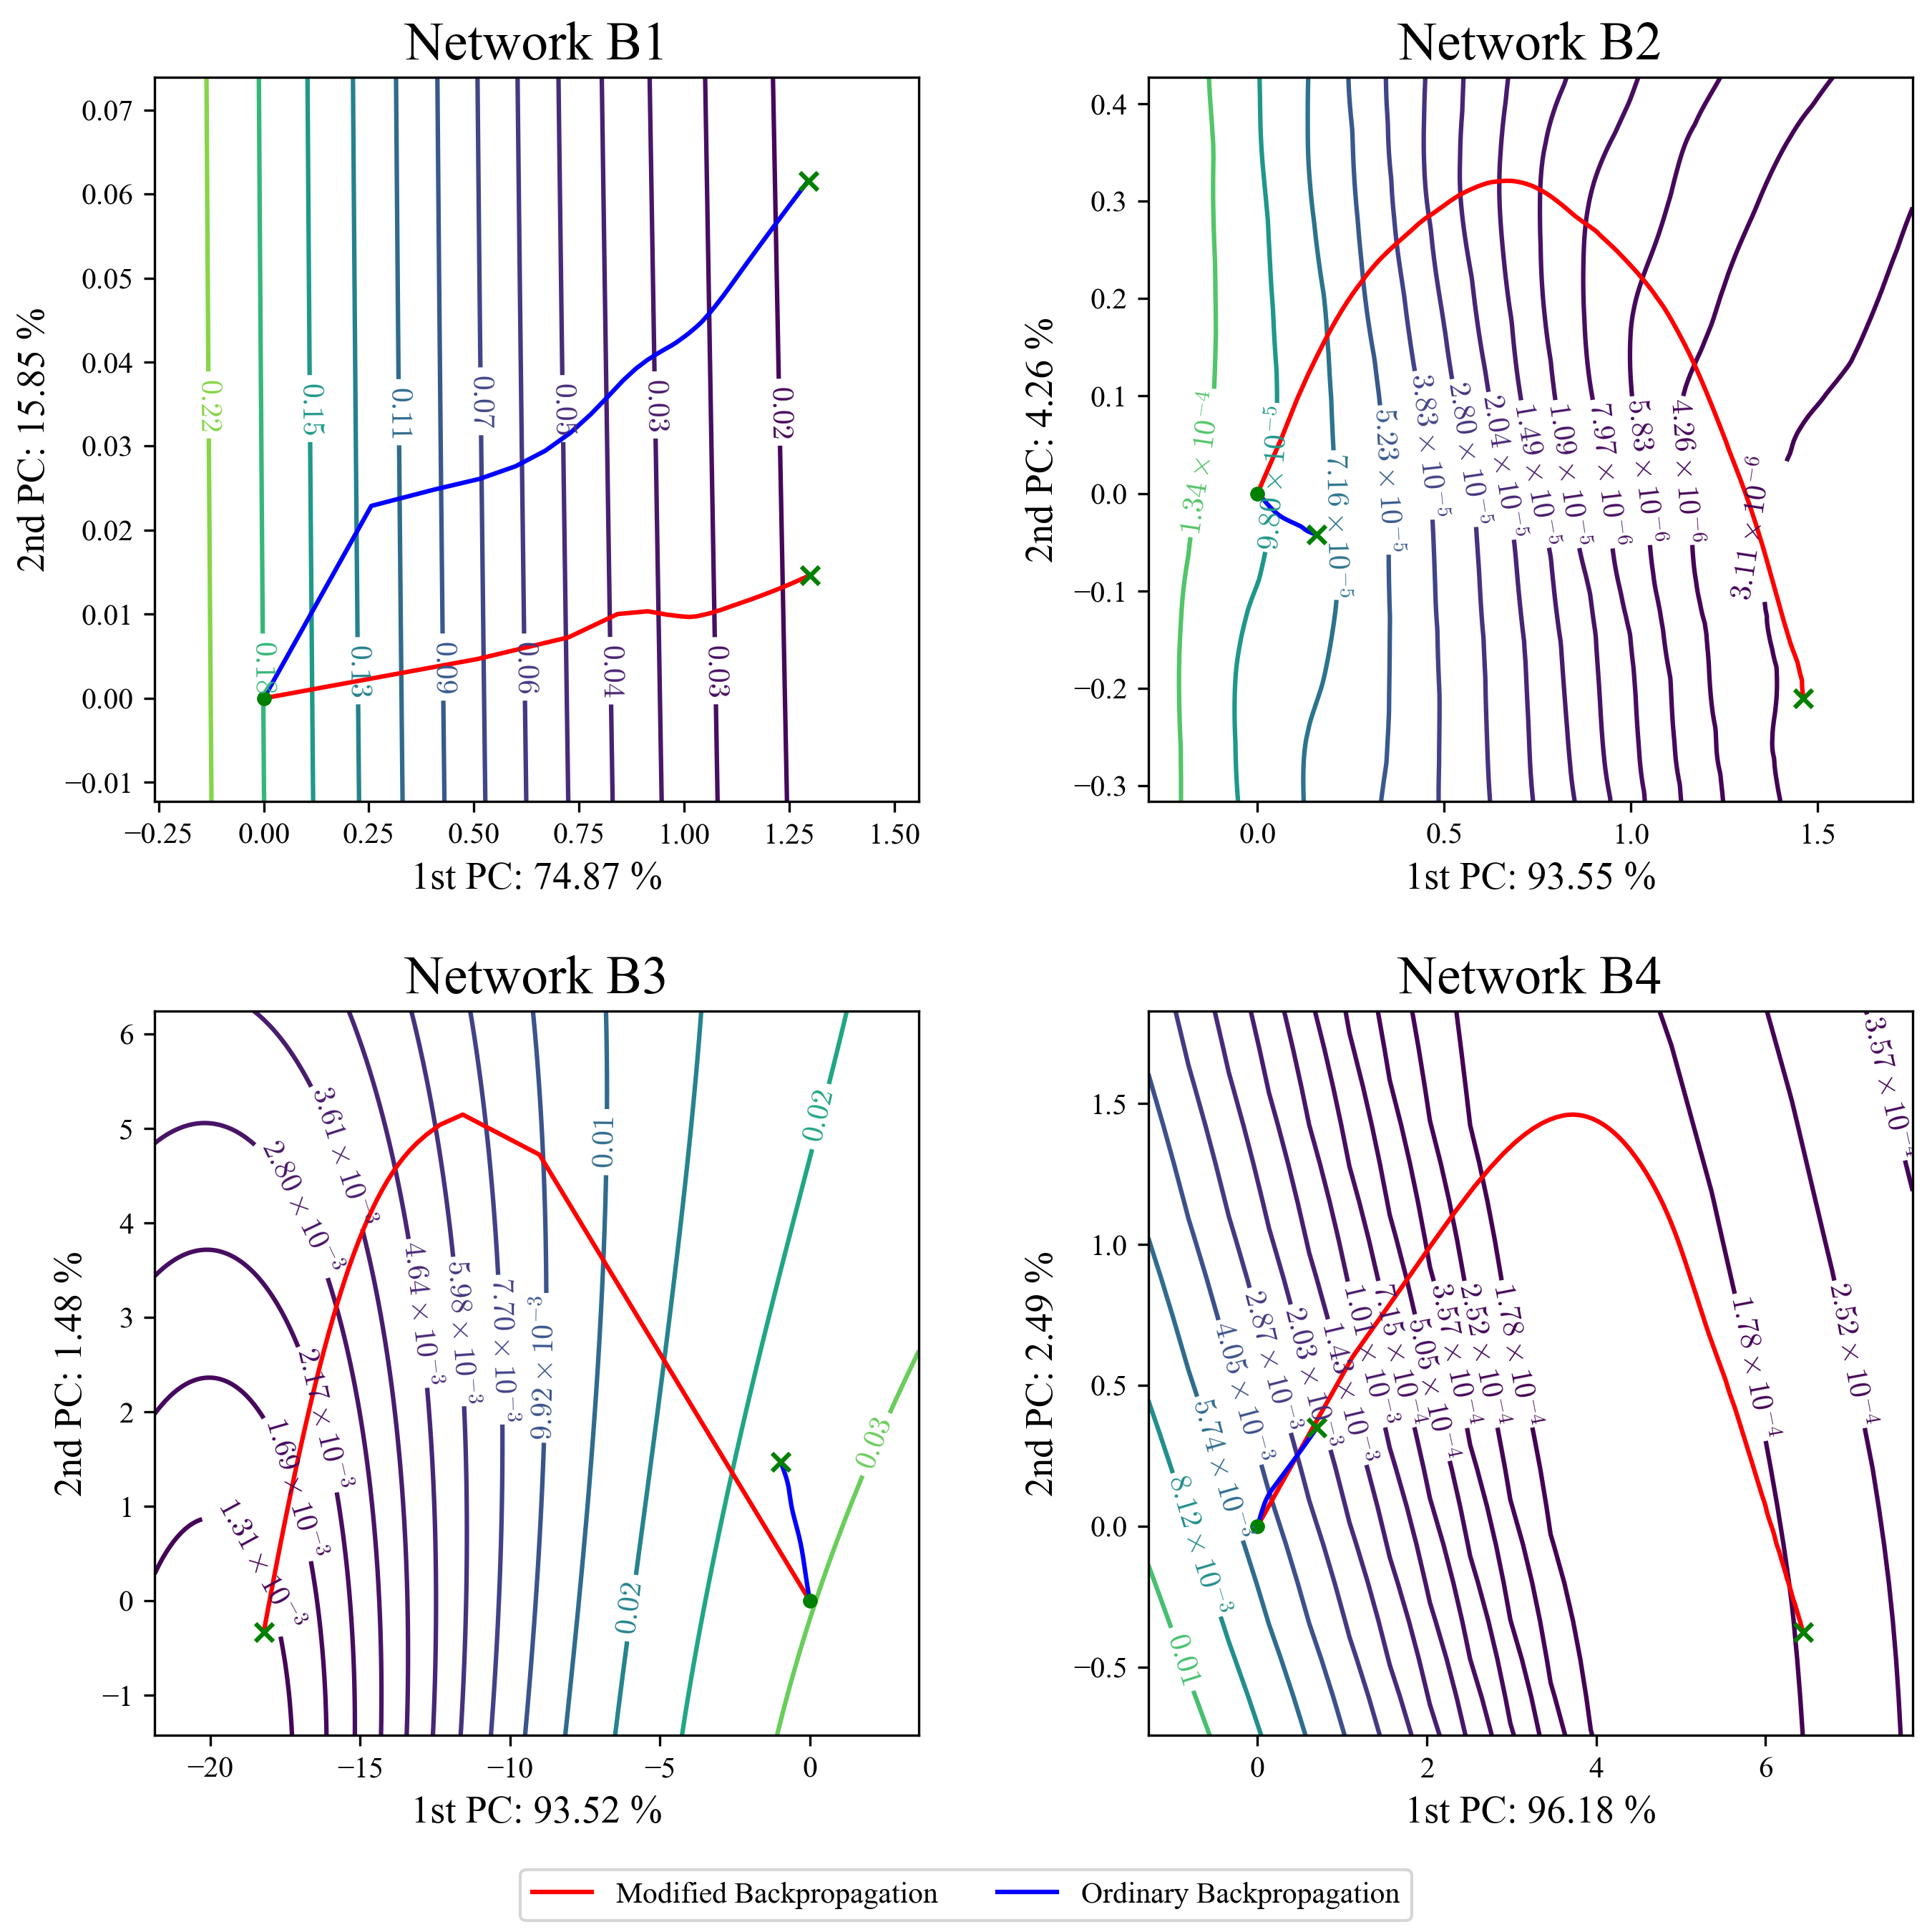
\includegraphics[width=\textwidth]{./resources/pca_all.png}
    \label{fig:big-pca}
    \caption{Representative runs with PCA analysis and optimizer trajectory in the projected space.}
\end{figure}

\end{document}


% This document was modified from the file originally made available by
% Pat Langley and Andrea Danyluk for ICML-2K. This version was created
% by Iain Murray in 2018, and modified by Alexandre Bouchard in
% 2019 and 2021 and by Csaba Szepesvari, Gang Niu and Sivan Sabato in 2022.
% Modified again in 2023 and 2024 by Sivan Sabato and Jonathan Scarlett.
% Previous contributors include Dan Roy, Lise Getoor and Tobias
% Scheffer, which was slightly modified from the 2010 version by
% Thorsten Joachims & Johannes Fuernkranz, slightly modified from the
% 2009 version by Kiri Wagstaff and Sam Roweis's 2008 version, which is
% slightly modified from Prasad Tadepalli's 2007 version which is a
% lightly changed version of the previous year's version by Andrew
% Moore, which was in turn edited from those of Kristian Kersting and
% Codrina Lauth. Alex Smola contributed to the algorithmic style files.
